\errorcontextlines=9999
\documentclass[
   aspectratio=169, % default is 43
   10pt, % font size, default is 11pt
   % nosectionframes,
   uniqueslidenumber,
   sectiontitleslides,
   % handout,
   professionalfonts
]{beamer}

\usepackage[T1]{fontenc}
\usepackage[utf8]{inputenc}
\usepackage[sfdefault]{FiraSans}

\usepackage{stmaryrd}
\usepackage[vvarbb]{notomath}
\usepackage{FiraMono}
\usepackage{tikz,forest}
\usepackage{ccicons}
\usepackage{fontawesome}
\usepackage{csquotes}
\usepackage{multicol}
\usepackage{../simplebnf}
\usepackage{../abstract-interpretation-ltx/absint}
\makeatletter
\def\absint@reflab#1#2{#2}% we do not need labels here
\usetikzlibrary{arrows.meta,decorations.pathmorphing,fit,decorations.pathreplacing,backgrounds,matrix,shadows}
\pgfdeclarelayer{foreground}
\usepackage{tikzpingus}
\pgfsetlayers{very-background,background,main,middle,foreground}
\def\sbseries{\fontseries{sb}\selectfont}
\def\textsb#1{{\sbseries#1}}

\usepackage{../slide-template-uulm/fancybeamer} % use the fancy beamer package
\usepackage{../slide-template-uulm/fancyuulm}
\setpaths{{../slide-template-uulm/}{../slide-template-uulm/logos/}{../slide-template-uulm/empty-slides/}{../xlistings/}}

\usepackage[auto]{contour}
\PassOptionsToPackage{normalem}{ulem}
\usepackage{ulem}
% we do it manually to "fix" it, we do not need breaking
\DeclareRobustCommand*\fancyul[2][\fancyulbackground]{%
   \def\fancyul@background{#1}%
   \def\ULdepth{1pt}%
   \def\ULthickness{.1ex}%
   \contourlength{.35pt}%
   {\color{\fancyulcolor}\uline{\phantom{#2}}}\llap{\contour\fancyul@background{#2}}%
}
\def\fancyulbackground{white}%
\colorlet{ul@line@color}{red!30!white}
\hypersetup{colorlinks=false,pdfborder=0 0 0}% just make sure :D
\def\fancyulcolor{ul@line@color}%
% we make the auto detection of the depth bigger
\def\update@ul{\setbox\z@\hbox{{(j}}\let\ULdepth\p@\edef\ULthickness{\the\dimexpr.235\dp\z@}}
% define a link macro that can be used with href and fancyul
\DeclareRobustCommand*\link{\hyper@normalise\link@do}
\def\link@do#1#2{\leavevmode\hskip-2\p@\href{#1}{\update@ul\hskip2\p@\fancyul{#2}}}% thinspace for some nicer padding
\DeclareRobustCommand*\hlink{\hyper@normalise\hlink@do}
\def\hlink@do#1#2{\leavevmode\hskip-2\p@\hyperlink{#1}{\update@ul\hskip2\p@\fancyul{#2}}}%


\usepackage{../code-animation/code-animation}
\usepackage[fakeminted,print]{../xlistings/xlistings}
\usepackage{multirow}
\xlstsetmintedstyle{plain}
\LoadLanguages{R,Java,yaml,C}
\lstcolorlet{keywordA}{black!70!red}%
\lstcolorlet{keywordB}{black!70!red}%
\lstcolorlet{keywordC}{black!70!red}%
\lstcolorlet{numbers}{black!70!yellow}%
\def\absintstyle#1{#1}
\xlstmintedwithlangbadge

% bib
\usepackage[style=alphabetic,backend=biber]{biblatex}
\addbibresource{./references.bib}

\DeclareCiteCommand{\fullcite}
  {\usebibmacro{prenote}}
  {%
      \usebibmacro{author}%
      \setunit{\labelnamepunct}\newblock
      \printfield[titlecase]{title}
      \space
      \newblock(\printlist{publisher}%
      \setunit{\addcomma\space}%
      \printfield{year})%
  }
  {\multicitedelim}
  {\usebibmacro{postnote}}

\newsavebox\SimpleSignLattice
\begin{lrbox}{\SimpleSignLattice}
\scriptsize
\begin{tikzpicture}[line cap=round,x=6.5mm,y=6.5mm]
   \node (top) at (0,0) {\absexpr{\top}};
   \node (pos) at (-1,-1) {\absexpr{\geq 0}};
   \node (neg) at (1,-1) {\absexpr{\leq 0}};
   \node (zero) at (0,-2) {\absexpr{0}};
   \node (bot) at (0,-3) {\absexpr{\bot}};
   \draw (top) -- (pos) -- (zero) -- (neg) -- (top) (zero) -- (bot);
\end{tikzpicture}
\end{lrbox}

\def\LeftArrow{\text{\BeginAccSupp{method=escape,ActualText={<-}}\(\leftarrow\)\EndAccSupp{}}}
\def\RightArrow{\text{\BeginAccSupp{method=escape,ActualText={->}}\(\rightarrow\)\EndAccSupp{}}}
\def\DoubleLeftArrow{\text{\BeginAccSupp{method=escape,ActualText={<<-}}\(\twoheadleftarrow\)\EndAccSupp{}}}
\def\DoubleRightArrow{\text{\BeginAccSupp{method=escape,ActualText={->>}}\(\twoheadrightarrow\)\EndAccSupp{}}}
\lstset{add to literate={<-}{{{\!\LeftArrow\!}}}2
   {<<-}{{{\!\DoubleLeftArrow\!}}}2
   {->}{{{\!\RightArrow\!}}}2
   {->>}{{{\!\DoubleRightArrow\!}}}2
}
\makeatletter
\def\ca@Strut{%
    \vphantom{%
        \xlst@font@fs@normal\xlst@styles@lst@basic\strut
    }%
}

\def\supercite#1{\raisebox{-1pt}{\textsuperscript{\footnotesize\color{gray}\cite{#1}}}}

\def\AbstractInfo#1{\ensuremath{\mathcolor{gray}{\Lbag}\,#1\,\mathcolor{gray}{\Rbag}}}
\def\Set#1{\ensuremath{\{#1\kern1pt\}}}
\def\IntCC#1#2{\ensuremath{[#1\,..\,#2]}}
\def\IntOC#1#2{\ensuremath{(#1\,..\,#2]}}
\def\IntCO#1#2{\ensuremath{[#1\,..\,#2)}}
\def\IntOO#1#2{\ensuremath{(#1\,..\,#2)}}
\def\S#1{\savebox\TestBox{\footnotesize\absexpr{\Set{#1}}}\ifdim\ht\TestBox>5mm\makebox[5mm][c]{\usebox\TestBox}\else\usebox\TestBox\fi}%
\def\I#1#2{\footnotesize\absexpr{\IntCC{#1}{#2}}}

\tikzset{
    path image shift/.style={}, % scale patch just for white padding
    path image/.style={path picture={\node[scale=.98] at ([path image shift]path picture bounding box.center) {#1};}}
}

\title[Static Analysis]{A Primer on Static Code Analysis}
\subtitle[SQA]{Software Quality Assurance --- Static Code Analysis, I}
\author[F. Sihler]{Florian Sihler}
\date{December 3, 2025}

\fancylogos{sp,uulm}

\usepackage{../beamer-latex-pdfpc-notes}
\urlstyle{same}


% TODO: take perspectives slide from thing for tubs
\begin{document}

\maketitle[titleimage/title][20]

\mode
<handout>

\begin{frame}{Outline}
% \begin{multicols}{2}
\tableofcontents[hideallsubsections]
% \end{multicols}
\end{frame}

\mode
<all>

\section{A first Overview}
\tikzset{
   RectRounding/.style={rounded corners=3pt},
   RawRect/.style={
      draw=black,
      rectangle,
      RectRounding,
      minimum size=1.8em,
      inner sep=5pt,
      fill=white,
   },
   Rect/.style={
      draw=black,
      rectangle,
      RectRounding,
      outer sep=2pt,
      minimum size=1.8em,
      fill=white,
      drop shadow={fill=lightgray!50}
   },
   Soft/.style={line join=round,line cap=round},
   Link/.style={
      draw,
      Soft,
      rounded corners=2.5pt,
      -Kite
   },
   na/.style={midway,above,font=\scriptsize,align=center},
   base@l/.style 2 args={edge node={node[na,#2]{#1}}},
   l/.style={base@l={#1}{}},
   lr/.style={base@l={#1}{right,align=left}},
   ll/.style={base@l={#1}{left,align=right}},
   lb/.style={base@l={#1}{below}},
}
\newsavebox\Landscape
\begin{frame}{Embedding a Landscape}
\begin{lrbox}{\Landscape}   
\begin{tikzpicture}[
   Rect/.append style={minimum height=3.25em,text width=6.5em,align=center}
]
   \node[Rect] (req) at (0,0) {Requirements};
   \node[Rect,right=1.5cm] (var) at (req.east) {Variability\\Req.};
   \node[Rect,right=1.5cm] (form) at (var.east) {Formal\\Req.};
   \node[Rect,below=6mm] (source) at(var.south) {Source\\Code};
   \path (req) -- (var) coordinate[pos=.5] (r2v);
   \path (var) -- (form) coordinate[pos=.5] (v2f);
   \node[Rect,below=6mm] (gui) at([xshift=-3.5mm]source.south-|r2v) {GUI Test\\Cases};
   \node[Rect,below=6mm] (test) at([xshift=3.5mm]source.south-|v2f) {Test\\Cases};
   \draw[Link] (req) to[l={Modeling}] (var);
   \draw[Link] (req.north) -- ++(0,3.5mm) to[l={Modeling/Formalization (Statecharts,~\ldots)}] ([yshift=3.5mm]form.north) -- (form.north);
   \draw[Link] ([yshift=-2mm]form.north east) -- ++(3mm,0) to[lr={Model\\Checking}] ([yshift=2mm,xshift=3mm]form.south east) -- ([yshift=2mm]form.south east);
   \draw[Link] (form.south) |- (test) node[na,pos=.25,right,align=left] {Model-Based Test\\Case Generation};
   \draw[Link] (var) -| (test) node[na,pos=.75,right,align=left] {Feature\\Interaction\\Testing};
   \draw[Link] (test.160) -| ([xshift=-8.5mm]source.south east) node[na,pos=.25,below] {Tests};
   \draw[Link] (gui.20) -| ([xshift=8.5mm]source.south west) node[na,pos=.25,below] {Tests};
   \draw[Link] (gui) -| (req.south) node[na,pos=.75,left,align=right] {Automated\\User-Interface\\Testing};
   \draw[Link,Kite-] ([yshift=-2mm]req.north west) -- ++(-3mm,0) to[ll={Dep.\\Req.}] ([yshift=2mm,xshift=-3mm]req.south west) -- ([yshift=2mm]req.south west);
   \draw[Link] (req.300) |- (source) node[na,pos=.75,below] {Implementation};
   \draw[Link] ([xshift=-2mm]test.south east) -- ++(0,-3mm) to[lb={Mutation, Property-Based,\\Prioritization}] ([xshift=2mm,yshift=-3mm]test.south west) -- ([xshift=2mm]test.south west);
   \tikzset{@/.style={}}
   \only<3->{
      \tikzset{@/.style={red,thick,font=\bfseries}}
   }
   \draw[Link,Kite-,@] ([xshift=-8.5mm]source.north east) -- ++(0,3.5mm) 
      -- ([xshift=8.5mm,yshift=3.5mm]source.north west) 
         node[na,yshift=-1.85mm,pos=1,left,align=right] (s) {~~~\strut Static}
         node[na,yshift=-1.85mm,pos=0,right,align=left] (a) {\,\strut Analysis}
      -- ([xshift=8.5mm]source.north west);
   \only<3->{
      \pgfonlayer{background}
      \node[fit={(s)(a)(source)},inner sep=1.5pt,draw,red,very thick,rounded corners=2pt,inner ysep=2.5pt,yshift=-1pt,fill=red!5] {};
      \endpgfonlayer
   }
\end{tikzpicture}
\end{lrbox}
\begin{tikzpicture}[overlay,remember picture]
   \onslide<2->{\node[yshift=-5mm] at(current page.center) {\usebox\Landscape};}
\end{tikzpicture}
\end{frame}

\newsavebox\PinguBox
\savebox\PinguBox{\tikz{\pingu[right wing shock, left eye wink, body type=legacy,left wing wave,name=pingu,heart]; \node[above] at (pingu-wing-left-tip) {\huge\faQuestion};}}
\newsavebox\PinguBoxB
\savebox\PinguBoxB{\tikz{\pingu[right wing shock, eyes shiny, body type=legacy,tie=pingu@purple,left wing wave,name=pingu,heart]; \node[above] at (pingu-wing-left-tip) {\huge\faQuestion};}}
\begin{frame}{}

\begin{tikzpicture}[overlay,remember picture]
   \def\shiftup{12mm}
   \only<9->{\def\shiftup{28mm}}
   \onslide<2->{\node[right=4mm,yshift=\shiftup] (@) at (current page.west) {\scalebox{.65}{\usebox\PinguBox}};}
   \onslide<3->{
      \node[below right,yshift=-2.5mm,xshift=2mm] (@) at (@.north east) {\textbf{\large What} is static {\only<4->{\color{lightgray}}code} analysis?};
   }
   \onslide<5->{
      \node[below=12.75mm,align=center,font=\large] at(current page.center|-@.south) {Discover \textit{\subnode{desc@syntactic-properties}{syntactic}/\subnode{desc@semantic-properties}{semantic} properties} of programs\\\subnode{desc@no-execute}{\textsb{without}} running them.\rlap{\supercite{rival2020introduction}}};
   }
   \onslide<6->{
      \draw[gray,Link] (desc@syntactic-properties.north) to[out=80,in=180] ++(7mm,11mm) node[below right,yshift=.6\baselineskip,align=left,font=\small] {%
         % syntactic:
         Derivable purely on program syntax.\\[-3.5pt]
         \scriptsize e.g., Line-Counts, Indentation, Parameter-Counts, \ldots
      };
   }
   \onslide<7->{
      \draw[gray,Link] (desc@semantic-properties.north) to[out=80,in=180] ++(7mm,4.5mm) node[below right,yshift=.6\baselineskip,align=left,font=\small] {%
         % semantic:
         Derivable from program semantics (behavior).\\[-3.5pt]
         \scriptsize e.g., Possible Variable Values, Termination,~\ldots
      };
   }
   \onslide<8->{
      \draw[gray,Link] (desc@no-execute) to[out=270,in=180] ++(7mm,-7.75mm) node[below right,yshift=.6\baselineskip,align=right,font=\small] {%
         Reason on \textit{all} possible executions.
      };
   }
   \onslide<10->{
      \node[right=4mm,yshift=-17mm] (@b) at (current page.west) {\scalebox{.65}{\usebox\PinguBoxB}};
      \node[below right,yshift=-2.5mm,xshift=2mm] (@b) at (@b.north east) {\textbf{\large Why} do static analysis?};
   }
   \onslide<11->{
      \node[below=10.75mm,text width=10cm,align=center,font=\footnotesize] at(current page.center)
      {%
      \begin{multicols}{2}
         % ask which they know?
         \begin{itemize}
            \item Find bugs or vulnerabilities
            \item<12-> Prove correctness
            \item<13-> Find and apply optimizations
            \item<14-> Follow \rlap{coding guidelines\,/\,style guides}
            \item<15-> Refactoring support
            \item<16-> \ldots\hfill\llap{\textcolor{lightgray}{(it is fun!)}}
         \end{itemize}
      \end{multicols}
      };
   }
\end{tikzpicture}
\end{frame}

\tikzfading[name=rectangular fade,
  inner color=transparent!0,
  middle color=transparent!0,
  outer color=transparent!100]

\newsavebox\CurrImgBox
\def\ImageWithRoundedCorners#1#2{%
   \savebox\CurrImgBox{\includegraphics[width=#1]{#2}}%
   \tikz{%
      \foreach \i/\o in {1/1,2/.5} {%
         \path[
            path image shift={(0pt,0pt)},
            path image={#2}{#1},
            rounded corners=8pt,
            path fading=rectangular fade,
            fading transform={xscale=1.2,yscale=1},
            draw,thin,white,
            opacity=\o
         ] (0,0) rectangle (\wd\CurrImgBox,\ht\CurrImgBox);%
      }
   }%
}
\setlength{\XeTeXLinkMargin}{0pt}
\tikzset{
   % https://tex.stackexchange.com/a/451914
   href node/.style={
        alias=sourcenode,
        append after command={
            let \p1= (sourcenode.north west),
                \p2= (sourcenode.south east),
                \n1={\x2-\x1},
                \n2={\y1-\y2} in
            node [inner sep=-0.5\pgflinewidth,outer sep=0pt,anchor=center, at=(sourcenode.center)] {\href{#1}{\XeTeXLinkBox{\phantom{\rule{\n1}{\n2}}}}}
        }
    },
   path image shift/.style={},
   path image/.style 2 args={path picture={\node at ([path image shift]path picture bounding box.center) {\includegraphics[width=#2]{#1}};}},
}


\savebox\PinguBox{%
   \tikz{\pingu[%
      eyes wink,
      wings wave,
      magnifier left,
      glasses,
      pants=pingu@red,
      pants bands
   ]}
}

\newsavebox\EdsgerDijkstra
\savebox\EdsgerDijkstra{%
\ImageWithRoundedCorners{17.25mm}{edsger-dijkstra.jpg}%
}

\begin{frame}{Let's find some bugs!}
\begin{tikzpicture}[overlay,remember picture]
   \def\shiftleft{0mm}
   \only<11->{\def\shiftleft{-40mm}}
   \onslide<2->{
      \node[align=center] (@) at([yshift=-5.25mm,xshift=\shiftleft]current page.center) {\scalebox{.65}{\usebox\PinguBox}\\Let's test!~\strut};  
   }
   \onslide<3->{
      \node[above right,xshift=-9mm] at(@.north east) {\large Dynamic};
   }
   \onslide<4->{
      \node[below right,xshift=-1mm] at(@.east) {\large Practical};
   }
   \onslide<5->{
      \node[above left] at(@.south west) {\large Quick};
   }
   \onslide<6->{
      \node[left] at(@.north west) {\large Easy};
   }
   \onslide<7->{
      \fill[white,opacity=.75] (@.center) circle[radius=3cm];
      \node[yshift=-2mm] at(@.north) {\huge But\only<8->{\rlap{\smash{,}}}};
   }
   \onslide<8->{
      \node[yshift=2mm] at(@) {\huge Tests are};
      \node[yshift=6mm] (@inc) at(@.south) {\huge\bfseries Unsound!};
   }
   \onslide<9->{
      \tikzset{@/.style={}}
      \only<10->{\tikzset{@/.style={opacity=.35}}}
      \node[below,@] (@sout) at(@inc.south) {\textit{System.out.println}?};
   }
   \onslide<10->{
      \node[lightgray,below=-3mm] at(@sout.south) {\itshape\bfseries Nope};
   }
   \onslide<12->{
      \node[right=.5mm,align=center,text width=7cm,yshift=-4.5mm,font=\large] at(current page.center) {\enquote{Program testing can be used to show the presence of bugs, but never to show their absence!}\\[2pt]\normalsize\citeauthor{dijkstra1969notes}\rlap{\supercite{dijkstra1969notes}}};
   }
   \onslide<13->{
      \node[below left=2.5mm,align=right,font=\tiny,
         href node={https://doi.org/10.1145/1787234.1787249}
      ] at(current page.north east) {%
         \usebox\EdsgerDijkstra\\[1.65pt]
         \textsb{Edsger W. Dijkstra} (1930--2002)\\
         \color{gray}Communications of the ACM
      };
   }
\end{tikzpicture}
\end{frame}

\usetikzlibrary{backgrounds,graphs,arrows.meta,decorations.pathreplacing}
\definecolor{BaseGray}{RGB}{66,66,66} % rgb(66,66,66)

\colorlet{SoftGray}{BaseGray!40}
\colorlet{BackGray}{BaseGray!5}
\colorlet{SoftTextGray}{BackGray!60!SoftGray}

\tikzset{
   FunctionDef/.style={
      draw=BaseGray,
      fill=BaseGray,
      minimum width=1.55cm,
      minimum height=1cm,
      text=white,
      font=\bfseries,
      text centered,
      inner sep=0pt,
      rounded corners=1mm,
      outer sep=2pt
   },
   Blob/.style={
      draw=SoftGray,
      fill=SoftGray,
      minimum size=4mm,
      text=white,
      circle,
      font=\bfseries,
      text centered,
      inner sep=0pt,
      outer sep=2pt
   },
   Def/.style={
      Blob,
      rectangle, rounded corners=1mm
   },
   ActiveBlob/.style={
      Blob,
      draw=BaseGray!80!white, fill=BaseGray!80!white
   },
   FunctionBack/.style={
      fill=BackGray,
      % draw=SoftGray,
      rounded corners=2mm,
      rectangle
   },
   Link/.style={
      draw=SoftGray,
      line width=1.5pt,
      line cap=round,
      line join=round,
      -%
   },
   FuncLink/.style={
      Link,
      draw=SoftGray,
      dotted
   },
   Cursor/.style={
      fill=BackGray,
      draw=BaseGray,
      line join=round,
      line cap=round
   },
   Hover-Over/.style={
      fill=BackGray,
      draw=SoftGray,
      opacity=.5,
      draw opacity=1,
      rounded corners=1mm,
      line join=round,
      line cap=round
   },
   Line-Of-Text/.style={
      fill=#1,
      draw=none,
      rounded corners=1.5pt,
      inner sep=1pt,
      minimum width=1cm,
      minimum height=6.5pt
   },
   Input-Base/.style={
      fill=BackGray,
      draw=SoftGray,
      rounded corners=1mm,
      inner sep=1pt,
      minimum width=2cm,
      minimum height=12pt
   },
   % code sub-styles
   A/.style={Line-Of-Text=SoftTextGray},
   B/.style={},
   C/.style={Line-Of-Text=SoftGray},
}

\newcommand\Back[4][]{
   \pgfonlayer{background}
   \fill[FunctionBack,#1] ([xshift=-2mm,yshift=-2mm]#2.south west) rectangle ([xshift=2mm,yshift=2mm]#3.north east);
   \coordinate (#4@north) at([yshift=2mm]0,0|-#3.north);
   \coordinate (#4@west) at([xshift=-2.5mm]0,0-|#2.west);
\endpgfonlayer
}
\newsavebox\UiBox
\begin{lrbox}{\UiBox}
\begin{tikzpicture}
   \node[FunctionDef] (F) at (0,0) {};

   \scope[shift={(F.south)},yshift=-1.5cm]
      \node[Def] (a1) at (-1,0) {};
      \node[Blob] (b1) at (.5,-.25) {};
      \node[ActiveBlob] (c1) at (1.55,-1.35) {};
      \node[Blob] (d1) at (-0.5,-1.6) {};
      \node[Blob] (e1) at (1.8,.25) {};
      \node[Blob] (f1) at (-2.2,-1.5) {};

      \graph[edges={Link}] {
         (a1) -> { (b1), (c1) } -> (d1) -> (e1) -> (a1),
         (f1) -> { (a1), (d1) }
      };

      \Back{f1}{e1}{f1}

      \draw[FuncLink] (f1@north) -- (F.south);
   \endscope

   \node[Blob] (a) at (2.5,0) {};
   \node[Blob] (b) at (1.5,1) {};
   \node[Blob] (c) at (3,2) {};
   \node[Blob] (d) at (-2.5,0.5) {};
   \node[Def] (e) at (-2.5,1.5) {};
   \node[Blob] (f) at (-3,2.5) {};
   \node[Blob] (g) at (-3.5,-1) {};
   \node[Blob] (h) at (-3,-2.5) {};

   \node[FunctionDef] (F2) at(5,-.5) {};
   \node[Blob] (u) at(5.5,1) {};

   \scope[shift={(F2.east)},xshift=1.5cm]

      \node[Blob] (a2) at (0,1.15) {};
      \node[Def] (b2) at (.75,1.85) {};
      \node[Blob] (c2) at (-.5,-.85) {};

      \node[Blob] (d2) at (1.33,0.25) {};
      \node[FunctionDef] (e2) at (2,-.75) {};

      \node[Blob] (f2) at (3.75,1.5) {};
      \node[Blob] (g2) at (2.75,2.5) {};

      \scope[shift=(e2.south), yshift=-1cm]
         \node[ActiveBlob] (a3) at (-1,0) {};
         \node[Blob] (b3) at (1,0) {};
         \draw[Link] (a3) -- (b3);
         \Back[white]{a3}{b3}{a3} % for coordinate
      \endscope

      \coordinate (ll) at ([yshift=-2mm]a3.south west-|c2.west);
      \coordinate (ur) at (f2.north east|-g2.north);

      \Back{ll}{ur}{e2}
      \draw[FuncLink] (e2@west) -- (F2.east);

      % draw inner later
      \Back[white]{a3}{b3}{xx} % for the overlay :D
      \draw[FuncLink] (a3@north) -- (e2.south);

      \graph[edges={Link}] {
         (a2) -> (b2) -> { (c2) , (d2) },
         (d2) -> { (e2), (f2) },
         (f2) -> (g2),
         (c2) -> (a3)
      };
   \endscope

   \graph[edges={Link}] {
      (F) -> { (a), (b) },
      (a) -> (e1),
      (b) -> (c) -> (b2),
      (b) -> (d) -> { (F), (e) },
      (e) -> (f) -> (c),
      (d) -> (g) -> (h) -> (f1),
      (u) -> (F2)
   };

   \coordinate (cursor-pos) at ([xshift=-1.65mm,yshift=2mm]F2.south east);
   \draw[Cursor,rotate around={28:(cursor-pos)}]  [rounded corners=2.25pt] (cursor-pos)  [rounded corners=2.25pt] -- ++(4pt,-9.5pt) [rounded corners=2pt] -- ++(-4pt,3pt) [rounded corners=2.25pt]-- ++(-4pt,-3pt) -- cycle;
   \node[below left,xshift=-1mm,yshift=1.15mm,Hover-Over,minimum width=1.25cm,minimum height=6mm] (hoverover) at(cursor-pos) {%
      %
   };
   % \scope[opacity=.95,transparency group]
      \fill[Line-Of-Text=SoftGray] ([shift={(2pt,-2pt)}]hoverover.north west) rectangle ++(7.5mm,-4pt);
      \fill[Line-Of-Text=SoftTextGray] ([shift={(2pt,-7.5pt)}]hoverover.north west) rectangle ++(11mm,-3pt);
      \fill[Line-Of-Text=SoftTextGray] ([shift={(2pt,-7.5pt-4.5pt)}]hoverover.north west) rectangle ++(8mm,-3pt);
   % \endscope

   % TODO: outsource window?
   \coordinate (wul) at ([shift={(-5mm,6mm)}]current bounding box.north west);
   \coordinate (wur) at ([shift={(5mm,6mm)}]current bounding box.north east);
   \draw[thin,rounded corners=3pt,SoftGray] ([shift={(-5mm,-5mm)}]current bounding box.south west) rectangle (wur);
   % just "overlay" the top :D
   \filldraw[SoftGray] ([yshift=-1mm]wul) coordinate (@) -- (wur|-@) [rounded corners] |- ([yshift=2.5mm]wul) [sharp corners] -- cycle;

   \fill[Line-Of-Text=BackGray] ([yshift=1.35mm,xshift=4pt]wul) rectangle ++(2cm,-1.27mm);
   \node[above left,BackGray] at([yshift=-1.33mm,xshift=-1mm]wur) {\smash{\scalebox{.9}{\scriptsize\faAngleDown~~\faAngleUp~~\faTimesCircle}}};

   \coordinate (root control window) at(current bounding box.south west);

   \scope[shift={(current bounding box.south east)},shift={(-7cm,4.5mm)}]
      \coordinate (wul) at (0,0);
      \coordinate (wur) at (8.5,0);

      \draw[thin,rounded corners=3pt,SoftGray,fill=white] (0,-5) rectangle (wur);

      % code line
      \draw[thin,BackGray] ([xshift=1cm,yshift=-1mm]wul) coordinate (@) -- (@|-0,-5);
      % line numbers and code
      \foreach[count=\i from 0] \Code in {
         {1/A,0.5/A,5/C,2/A},
         {1.5/B,3/A,0.5/A,2/A},
         {},
         {1.5/B,0.5/A,3/A},
         {1/A},
         {},
         {5/A,0.5/A,2/A},%
         {0.5/A,5/A,3/A,0.5/A,2/A,5.5/A},
         {},
         {1/C,0.5/A,1/A,0.5/A,1/A,0.5/A,0.15/B,0.5/A},
         {1.5/B,3/A,0.5/A,1/C,2/A,1.5/A,1/C,1.5/A},
         {1.5/B,0.75/A,0.5/A,1.5/A,0.5/A,1/A},
         {1.5/B,3/A,0.5/A,2/A},
         {1.5/B,2/A,0.5/A,2/A},
         {1/A}%
      } {
         \ifnum\i<6 \def\Width{4mm} \else \def\Width{6mm} \fi
         \fill[Line-Of-Text=BackGray] ([yshift=-1mm,xshift=8mm]wul|-0,-\i*0.33*10mm+1mm) rectangle ++(-\Width,-2mm);
         \def\XShift{5}
         \foreach \CW/\Style in \Code {
            \ifstrequal{\Style}{B}{\def\RandomSuffix{0}}{\def\RandomSuffix{(rand*0.4mm+0.75mm)}}
            \pgfmathsetmacro\w{3*\CW mm+\RandomSuffix}
            \path[\Style] ([yshift=-1mm,xshift=1cm+\XShift pt]wul|-0,-\i*0.33*10mm+1mm) rectangle ++(\w pt,-2mm);

            \pgfmathsetmacro{\XShift}{\XShift+\w pt+1.5mm}
            \xdef\XShift{\XShift}
         }
      }

      % slider
      \draw[Line-Of-Text=SoftTextGray,rounded corners=.325mm] ([yshift=-4cm+5mm,xshift=-1mm]wur) rectangle ++(-.75mm,-1cm);

      % just redraw the frame :D
      \draw[thin,rounded corners=3pt,SoftGray] (0,-5) rectangle (wur);

      \filldraw[SoftGray] ([yshift=-1mm]wul) coordinate (@) -- (wur|-@) [rounded corners] |- ([yshift=2.5mm]wul) [sharp corners] -- cycle;

      \fill[Line-Of-Text=BackGray] ([yshift=1.35mm,xshift=4pt]wul) rectangle ++(1.66cm,-1.27mm);
      \node[above left,BackGray] at([yshift=-1.33mm,xshift=-1mm]wur) {\smash{\scalebox{.9}{\scriptsize\faAngleDown~~\faAngleUp~~\faTimesCircle}}};

   \endscope

   % window for controls
   \scope[shift={(root control window)},shift={(-1cm,-5mm)}]
      \draw[thin,rounded corners=3pt,SoftGray,fill=white] (0,-4) rectangle ++(8.33cm,4cm);
      \coordinate (wul) at (0,0);
      \coordinate (wur) at (8.33,0);

      \node[Input-Base,minimum width=6cm,below right=3mm] (slice-criterion-input) at (wul) {};
      \fill[Line-Of-Text=SoftTextGray] ([yshift=1mm,xshift=4pt]slice-criterion-input.west) rectangle ++(1.25cm,-2mm);
      \fill[Line-Of-Text=SoftTextGray] ([yshift=1mm,xshift=4pt+1.25cm+2mm]slice-criterion-input.west) rectangle ++(1cm,-2mm);

      % frame stuff
      \filldraw[SoftGray] ([yshift=-1mm]wul) coordinate (@) -- (wur|-@) [rounded corners] |- ([yshift=2.5mm]wul) [sharp corners] -- cycle;
      \node[right=1mm,SoftGray,] at(slice-criterion-input.east) {\tiny\faChevronRight~~~~~\faPieChart~~\faUpload~~\faDownload};

      % logging window
      \draw[rounded corners=3pt,BackGray,fill=white] ([xshift=3mm,yshift=-1cm]wul) rectangle ([xshift=-3mm,yshift=-3.7cm]wur);

      % log
      \foreach[count=\i from 0] \Code in {
         {1/A,2/A,6/A,1/B,3/A},
         {1.5/B,3/A,2/A,2/A,1/A},
         {1.5/B,2/A,3/A,1/A,2/A,3/A,1/A},
         {1.5/B,4/A,1/A},
         {1.5/B,3/A,2/A,2/A,1/A},
         {1.5/B,3/A,1/A,4/A,1/A},
         {},
         {1/A,2/A,6/A},
         {1/A,2/A,3/A,1.5/A,2.5/A},
      } {
         \def\XShift{5}
         \foreach \CW/\Style in \Code {
            \ifstrequal{\Style}{B}{\def\RandomSuffix{0}}{\def\RandomSuffix{(rand*0.4mm+0.75mm)}}
            \pgfmathsetmacro\w{3*\CW mm+\RandomSuffix}
            \path[\Style] ([yshift=-2.5mm-1cm,xshift=3.25mm+\XShift pt]wul|-0,-\i*0.28*10mm+1mm) rectangle ++(\w pt,-1.75mm);

            \pgfmathsetmacro{\XShift}{\XShift+\w pt+1mm}
            \xdef\XShift{\XShift}
         }
      }

      % slider
      \draw[Line-Of-Text=SoftTextGray,rounded corners=.325mm] ([yshift=-2cm+3mm,xshift=-4mm]wur) rectangle ++(-.75mm,-1cm);

      % head
      \fill[Line-Of-Text=BackGray] ([yshift=1.35mm,xshift=4pt]wul) rectangle ++(5mm,-1.27mm);
      \fill[Line-Of-Text=BackGray] ([yshift=1.35mm,xshift=4pt+6.5mm]wul) rectangle ++(1cm,-1.27mm);
      \node[above left,BackGray] at([yshift=-1.33mm,xshift=-1mm]wur) {\smash{\scalebox{.9}{\scriptsize\faAngleDown~~\faAngleUp~~\faTimesCircle}}};
   \endscope
\end{tikzpicture}
\end{lrbox}
\newsavebox\CodeFile
\begin{lrbox}{\CodeFile}
\scalebox{1.45}{%

\begin{tikzpicture}
   \draw[rounded corners=1.5pt,fill=white] (0,0) |- ++(.6,-.8) [sharp corners] -- ++(0,.6) -- ++(-.2,.2) coordinate (@rl) [rounded corners=2pt] -- cycle (@rl) |- ++(.2,-.2);
   \draw[thick,line cap=round,lightgray] (.1,-.1) -- ++(.2,0)
      % for what have I written random code generation? :C 
      (.1,-.15) -- ++(.1,0) ++(.05,0) -- ++(.1,0)
      (.125,-.2) -- ++(.15,0)++(.05,0)--++(.025,0)
      (.1,-.25) -- ++(.3,0)
      (.125,-.3) --++(.2,0)++(.05,0)--++(.05,0)
      (.125,-.35) --++(.15,0)++(.05,0)--++(.1,0)
      (.15,-.4)--++(.2,0)
      (.15,-.4)--++(.1,0)++(.05,0)--++(.05,0)
      (.125,-.45)--++(.05,0)
      (.1,-.5)--++(.066,0)++(.05,0)--++(.15,0)
      (.1,-.6)--++(.15,0)++(.05,0)--++(.15,0)
      (.1,-.65)--++(.2,0)
      (.1,-.7)--++(.1,0)++(.05,0)--++(.15,0)
   ;
\end{tikzpicture}}
\end{lrbox}

\begin{frame}{\strut A First Look}
% they take input, textual, syntactical, semantic (call graphs, pdg, ...), metadata, historical information, requirements, annotations (types, contracts), ...
\vspace*{.5em}\hspace*{-3.5mm}
\begin{tikzpicture}[o/.style={outer sep=0pt,inner sep=0pt}]
   \onslide<2->{%
      \node[o] (@) at (0,0) {\usebox\CodeFile};
      \node[above=2.5mm,xshift=1.15mm,gray] at(@.north) {\tiny They take \textbf{\normalsize Input}};
   }
   \pgfonlayer{background}
   \onslide<2->{%
   \scope[transparency group,opacity=.4]
   \node[o,rotate around={-30:(@.south east)},anchor=south east] at(@.south east) {\usebox\CodeFile};
   \node[o,rotate around={-12:(@.south east)},anchor=south east] at(@.south east) {\usebox\CodeFile};
   \endscope}
   \endpgfonlayer
   \begin{uncoverenv}<3->
   \coordinate (@) at(@.east);
   \foreach[count=\i] \usecase/\targeti in {{\raisebox{1pt}{Textual}}/4,Syntactical/5, Semantical/6, Historical/7, Annotated/8, {\only<-9|handout:0>{\ldots}\only<10->{\raisebox{-3pt}{Metadata,~\ldots}}}/9} { % program spectra, hardware, contexts, ...
   \pgfmathsetmacro\rot{-24*\i+66}
      \onslide<\targeti->{
         \path ([xshift=.5mm]@.east)++(\rot+10:1mm) coordinate (@a);
         \fill[opacity=.18,gray] (@a.east) -- ++(\rot:1.5cm) arc (\rot:\rot+20:1.5cm) -- cycle;
         \draw[thick,gray] (@a.east)++(\rot:1.5cm) arc (\rot:\rot+20:1.5cm);
         \path (@a.east) -- ++(1.05*\rot+10:1.6cm) node[right,font=\small,darkgray] (@uc-\i) {\vphantom{a}\smash{\usecase}};
      }
   }
   \node[above=1.65mm,xshift=1mm,gray] (@perspective-label) at(current bounding box.north) {\tiny And use \textbf{\normalsize Perspectives} \rlap{(often combined)}};
   \end{uncoverenv}
   \onslide<11->{%
      \draw[Kite-,gray] ([xshift=6.25mm,yshift=-1mm]current bounding box.south) to[out=-90,in=0] ++(-4.5mm,-5mm) node[below left,yshift=.42\baselineskip,align=right,text width=2.5cm,font=\tiny] {Some of those are the result of other static or dynamic analyses};
   }
   \begin{uncoverenv}<12->
      \node[right,yshift=-2mm,xshift=1cm,align=left,font=\small,darkgray,text width=3.25cm] (@techn) at(current bounding box.east){{\onslide<13->{\subnode{tc-search}{Text/Code Search}\strut}}~\\[4mm]\strut{\onslide<14->{\subnode{clustering}{Clustering}}}~\\[4mm]\strut{\onslide<15->{\subnode{ai}{Abstract Domains}}}~\\[4mm]\strut{\onslide<16->{\subnode{df-constraints}{Dataflow Constraints}}}~\\[1mm]\strut{\onslide<16->{\centerline{\footnotesize\(\vdots\)}}}};
      \onslide<12->{
         \node[above=2.5mm,gray,xshift=-4.5mm] at(@techn.north) {\tiny To apply \textbf{\normalsize Theory}};
      }
   \end{uncoverenv}
   \scope[gray,line cap=round]
   \only<17->{
      \draw ([yshift=1.5pt]@uc-1.east) -- ([yshift=-2.5mm]@techn.north west);
      \draw ([yshift=1.5pt]@uc-2.east) -- ([yshift=-2.5mm]@techn.north west);
      \draw[densely dotted] ([yshift=1.5pt]@uc-3.east) -- ([yshift=-2.5mm]@techn.north west);
   }
   \only<18->{
      \draw ([yshift=1.5pt]@uc-1.east) -- ([yshift=-10.5mm]@techn.north west);
      \draw ([yshift=0pt]@uc-2.east) -- ([yshift=-10.5mm]@techn.north west);
      \draw ([yshift=1.5pt]@uc-4.east) -- ([yshift=-10.5mm]@techn.north west);
      
      \draw ([yshift=-1pt]@uc-2.east) -- ([yshift=-18.5mm]@techn.north west);
      \draw ([yshift=-1pt]@uc-3.east) -- ([yshift=-18.5mm]@techn.north west);
      \draw ([yshift=1.5pt]@uc-5.east) -- ([yshift=-18.5mm]@techn.north west);
      
      \draw ([yshift=-1pt]@uc-2.east) -- ([yshift=-26mm]@techn.north west);
      \draw ([yshift=-1pt]@uc-3.east) -- ([yshift=-26mm]@techn.north west);
   }
   \endscope
   \begin{uncoverenv}<19->
      
      \onslide<20->{\node[right=7.5mm] (@) at(current bounding box.east) {\resizebox*!{2.85cm}{\usebox\UiBox}};
      \scope[transparency group,opacity=.5,every path/.append style={line cap=round,line width=.5pt}]
         \draw[-Kite,gray] ([yshift=-2.5mm,xshift=-6.5mm]@techn.north east) to[out=0,in=180] ([xshift=1.5mm,yshift=-6.35mm]@.west);
         \draw[-Kite,gray] ([yshift=-10.5mm,xshift=-18.5mm]@techn.north east) to[out=0,in=180] ([xshift=7.15mm,yshift=-1.35mm]@.west);
         \draw[-Kite,gray] ([yshift=-18.5mm,xshift=-6.25mm]@techn.north east) to[out=0,in=180] ([xshift=26.15mm,yshift=-9.35mm]@.west);
         \draw[-Kite,gray] ([yshift=-26mm,xshift=-2.5mm]@techn.north east) to[out=0,in=180] ([xshift=26.15mm,yshift=-9.35mm]@.west);
      \endscope
      }
      \node[above, gray] at(@.north) {\tiny And \textbf{\normalsize Communicate} or \textbf{\normalsize Use} results};
   \end{uncoverenv}
\end{tikzpicture}
\end{frame}

\newsavebox\ASTStructure
\begin{lrbox}{\ASTStructure}
\begin{forest}
for tree={
   grow'=0,
   l=0pt,
   l sep-=5pt,
   s sep-=2pt,
   s=0pt,
   fit=band
}
[\bIndexR{<-}
   [\bIndexR{x}]
   [\bIndexR{*}
      [\smash{\raisebox{-4.25pt}{\bIndexR{sin}}}
         [\smash{\raisebox{-3.75pt}{\bIndexR{y}}}]
      ]
      [\bIndexR{z}]
   ]
]
\end{forest}
\end{lrbox}
\newsavebox\SemanticalStructure
\begin{lrbox}{\SemanticalStructure}
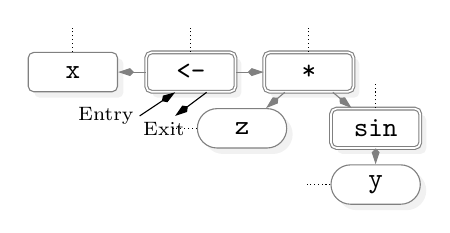
\begin{tikzpicture}[
   comm/.style={rectangle,draw=gray,text width=9mm,align=center,minimum height=5mm,font=\ttfamily,fill=white,fill opacity=1,drop shadow={fill=lightgray!42}},
   d/.style={comm,rounded corners=2pt}, % variable def
   u/.style={comm,rounded corners=2.5mm}, % variable use % rounded rectangle breaks anchors
   e/.style={comm,rounded corners=2.5mm,densely dotted,thick,fill=white}, % exit point
   fc/.style={comm,double,rounded corners=2pt},
]

   \node[fc] (assign) at (0,0) {\bIndexR{<-}};
   \node[d,left=3.5mm] (x-def) at(assign.west) {\bIndexR{x}};
   \node[fc,right=3.5mm] (mul) at(assign.east) {\bIndexR{*}};
   \node[u,below left=2mm,xshift=5mm] (z-use) at(mul.south west) {\bIndexR{z}};
   \node[fc,below right=2mm,xshift=-5mm] (sin) at(mul.south east) {\bIndexR{sin}};
   \node[u,below=2mm] (y-use) at(sin.south) {\bIndexR{y}};
   \draw[-Kite,gray] (assign) -- (x-def);
   \draw[-Kite,gray] (assign) -- (mul);
   \draw[-Kite,gray] (mul) -- (z-use);
   \draw[-Kite,gray] (mul) -- (sin);
   \draw[-Kite,gray] (sin) -- (y-use);
   \draw[densely dotted] (x-def.north) -- ++(0,3mm);
   \draw[densely dotted] (y-use.west) -- ++(-3mm,0);
   \draw[densely dotted] (z-use.west) -- ++(-3mm,0);
   \draw[densely dotted] (assign.north) -- ++(0,3mm);
   \draw[densely dotted] (sin.north) -- ++(0,3mm);
   \draw[densely dotted] (mul.north) -- ++(0,3mm);
   \draw[Kite-] ([xshift=-2mm]assign.south)
      -- ++(-4.5mm,-3mm) node[left] {\scriptsize Entry\!};
   \draw[-Kite] ([xshift=2mm]assign.south)
      -- ++(-4mm,-3mm) node[below=-.5mm] {\scriptsize Exit~~~~};
\end{tikzpicture}
\end{lrbox}
\newsavebox\HistoricalInfo
\begin{lrbox}{\HistoricalInfo}
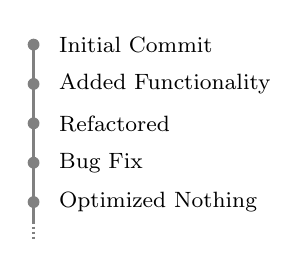
\begin{tikzpicture}
   \draw[thick,line cap=round,gray]
      (0,0) -- ++(0,-2.25cm);
   \draw[thick,densely dotted,gray]
      (0,-2.25cm) -- ++(0,-.25cm);
   \foreach \y/\label in {0/{Initial Commit},-5mm/{Added Functionality},-1cm/{Refactored},-1.5cm/{Bug Fix},-2cm/{Optimized Nothing}} {
      \fill[gray] (0,\y) circle (.75mm);
      \node[right=2mm] at (0,\y) {\footnotesize\label};
   }
\end{tikzpicture}
\end{lrbox}

\def\ShowBasicFlow{%
   \node[o] (@) at (0,0) {\usebox\CodeFile};
   \node[above=2.5mm,xshift=1.15mm,gray] at(@.north) {\tiny They take \textbf{\normalsize Input}};
   \pgfonlayer{background}
   \scope[transparency group,opacity=.4]
   \node[o,rotate around={-30:(@.south east)},anchor=south east] at(@.south east) {\usebox\CodeFile};
   \node[o,rotate around={-12:(@.south east)},anchor=south east] at(@.south east) {\usebox\CodeFile};
   \endscope
   \endpgfonlayer
   \coordinate (@) at(@.east);
   \coordinate (@inp) at(@);
   \foreach[count=\i] \usecase/\targeti in {{\raisebox{1pt}{Textual}}/4,Syntactical/5, Semantical/6, Historical/7, Annotated/8, {\raisebox{-3pt}{Metadata,~\ldots}}/9} { % program spectra, hardware, contexts, ...
   \pgfmathsetmacro\rot{-24*\i+66}
         \path ([xshift=.5mm]@.east)++(\rot+10:1mm) coordinate (@a);
         \fill[opacity=.18,gray] (@a.east) -- ++(\rot:1.5cm) arc (\rot:\rot+20:1.5cm) -- cycle;
         \draw[thick,gray] (@a.east)++(\rot:1.5cm) arc (\rot:\rot+20:1.5cm);
         \path (@a.east) -- ++(1.05*\rot+10:1.6cm) node[right,font=\small,darkgray] (@uc-\i) {\vphantom{a}\smash{\usecase}};
   }
   \node[above=1.65mm,xshift=1mm,gray] (@perspective-label) at(current bounding box.north) {\tiny And use \textbf{\normalsize Perspectives} \rlap{(often combined)}};
      \draw[Kite-,gray] ([xshift=6.25mm,yshift=-1mm]current bounding box.south) to[out=-90,in=0] ++(-4.5mm,-5mm) node[below left,yshift=.42\baselineskip,align=right,text width=2.5cm,font=\tiny] {Some of those are the result of other static or dynamic analyses};
      \node[right,yshift=-2mm,xshift=1cm,align=left,font=\small,darkgray,text width=3.25cm] (@techn) at(current bounding box.east){{{\subnode{tc-search}{Text/Code Search}\strut}}~\\[4mm]\strut{{\subnode{clustering}{Clustering}}}~\\[4mm]\strut{{\subnode{ai}{Abstract Domains}}}~\\[4mm]\strut{{\subnode{df-constraints}{Dataflow Constraints}}}~\\[1mm]\strut{{\centerline{\footnotesize\(\vdots\)}}}};
         \node[above=2.5mm,gray,xshift=-4.5mm] (@theory-label) at(@techn.north) {\tiny To apply \textbf{\normalsize Theory}};
   \scope[gray,line cap=round]
      \draw ([yshift=1.5pt]@uc-1.east) -- ([yshift=-2.5mm]@techn.north west);
      \draw ([yshift=1.5pt]@uc-2.east) -- ([yshift=-2.5mm]@techn.north west);
      \draw[densely dotted] ([yshift=1.5pt]@uc-3.east) -- ([yshift=-2.5mm]@techn.north west);
      \draw ([yshift=1.5pt]@uc-1.east) -- ([yshift=-10.5mm]@techn.north west);
      \draw ([yshift=0pt]@uc-2.east) -- ([yshift=-10.5mm]@techn.north west);
      \draw ([yshift=1.5pt]@uc-4.east) -- ([yshift=-10.5mm]@techn.north west);
      
      \draw ([yshift=-1pt]@uc-2.east) -- ([yshift=-18.5mm]@techn.north west);
      \draw ([yshift=-1pt]@uc-3.east) -- ([yshift=-18.5mm]@techn.north west);
      \draw ([yshift=1.5pt]@uc-5.east) -- ([yshift=-18.5mm]@techn.north west);
      
      \draw ([yshift=-1pt]@uc-2.east) -- ([yshift=-26mm]@techn.north west);
      \draw ([yshift=-1pt]@uc-3.east) -- ([yshift=-26mm]@techn.north west);
   \endscope
      \node[right=7.5mm] (@ui-box) at(current bounding box.east) {\resizebox*!{2.85cm}{\usebox\UiBox}};
      \scope[transparency group,opacity=.5,every path/.append style={line cap=round,line width=.5pt}]
         \draw[-Kite,gray] ([yshift=-2.5mm,xshift=-6.5mm]@techn.north east) to[out=0,in=180] ([xshift=1.5mm,yshift=-6.35mm]@ui-box.west);
         \draw[-Kite,gray] ([yshift=-10.5mm,xshift=-18.5mm]@techn.north east) to[out=0,in=180] ([xshift=7.15mm,yshift=-1.35mm]@ui-box.west);
         \draw[-Kite,gray] ([yshift=-18.5mm,xshift=-6.25mm]@techn.north east) to[out=0,in=180] ([xshift=26.15mm,yshift=-9.35mm]@ui-box.west);
         \draw[-Kite,gray] ([yshift=-26mm,xshift=-2.5mm]@techn.north east) to[out=0,in=180] ([xshift=26.15mm,yshift=-9.35mm]@ui-box.west);
      \endscope
      \node[above, gray] (@comm-label) at(@ui-box.north) {\tiny And \textbf{\normalsize Communicate} or \textbf{\normalsize Use} results};
}

\begin{frame}{\strut Perspectives}
\vspace*{.5em}\hspace*{-3.5mm}
\begin{tikzpicture}[o/.style={outer sep=0pt,inner sep=0pt}]
   \ShowBasicFlow
\onslide<2->{
   \node[fit={
      (@uc-1)
      (@uc-2)
      (@uc-3)
      (@uc-4)
      (@uc-5)
      ([yshift=-1mm]@uc-6.south)
      (@inp)
      (@perspective-label.north)
      ([xshift=14mm]@perspective-label.east)
      (@perspective-label.west)
   }] (@) {};
   \fill[white,opacity=.9,even odd rule]
      (current bounding box.south east)
         rectangle
      ([yshift=3mm]current bounding box.north west)
      (@.north west)
         rectangle
      (@.south east);
   \draw[ultra thick,red,rounded corners=6pt]
      (@.north west)
         rectangle
      (@.south east);
}
\pgfinterruptboundingbox
\onslide<3->{
   \node[above right,xshift=5mm,Rect,align=left] (@textual) at(@.north east) {\bIndexR{x <- sin(y) * z}};
   \node[below right,yshift=1mm] at(@textual.south west) {\scriptsize\textsb{Textual Perspective}};
}
\onslide<4->{
   \node[below right,xshift=12mm,yshift=-4.5mm,Rect,align=left] (@syntactical) at(@.north east) {\usebox\ASTStructure};
   \node[below right,yshift=1mm] at(@syntactical.south west) {\scriptsize\textsb{Syntactical Perspective} (AST)};
}
\onslide<5->{
   \node[below right,xshift=-7.5mm,yshift=-6mm,Rect,align=left] (@semantical) at(@syntactical.south west) {\usebox\SemanticalStructure};
   \node[below right,yshift=1mm] at(@semantical.south west) {\scriptsize\textsb{Semantical Perspective} (CFG\,\&\,DFG)};
}
\onslide<6->{
   \node[above right,Rect,xshift=2.75mm,yshift=3.5mm] (@historical) at(@syntactical.south east) {\usebox\HistoricalInfo};
   \node[below right,yshift=1mm] at(@historical.south west) {\scriptsize\textsb{Historical Perspective}};
}
\onslide<7->{
   \node[above right,Rect,xshift=2.75mm,yshift=18.5mm,align=left] (@annotated) at(@semantical.south east) {
      \scriptsize\textcolor{gray}{\figureversion{lf}\selectfont\#~Caused CVE 2025-12345}\\[-.5mm]
      \bIndexR{x <- sin(y)}
   };
   \node[below right,yshift=1mm] at(@annotated.south west) {\scriptsize\textsb{Annotated Perspective}};
}
\onslide<8->{
   \node[above right,Rect,xshift=2.75mm,yshift=-.5mm,align=left,font=\footnotesize] (@metadata) at(@semantical.south east) {
      Author: Jane Doe\\
      Code Review: Passed\\
      \ldots
   };
   \node[below right,yshift=1mm] at(@metadata.south west) {\scriptsize\textsb{Metadata Perspective}};
}
\endpgfinterruptboundingbox
\end{tikzpicture}
\end{frame}
\def\SoftBox#1#2#3{%
   \pgfsetfillopacity{.85}%
   \colorbox{#1!33!white}{%
      \pgfsetfillopacity{1}%
      \parbox{#2}{#3}%
      \pgfsetfillopacity{.85}%
   }\pgfsetfillopacity{1}%
}
\def\lab#1{%
   \raisebox{2pt}{\normalfont\scriptsize\color{gray}#1}%
}
\begin{frame}{\strut Theory}
\vspace*{.5em}\hspace*{-3.5mm}
\begin{tikzpicture}[o/.style={outer sep=0pt,inner sep=0pt}]
   \ShowBasicFlow
\onslide<2->{
   \node[fit={
      (@techn)
      (@theory-label.north)
      (@theory-label.west)
   }] (@) {};
   \fill[white,opacity=.9,even odd rule]
      (current bounding box.south east)
         rectangle
      ([yshift=3mm]current bounding box.north west)
      (@.north west)
         rectangle
      (@.south east);
   \draw[ultra thick,red,rounded corners=6pt]
      (@.north west)
         rectangle
      (@.south east);
}
\pgfinterruptboundingbox
\onslide<3->{
\node[above left=3mm,yshift=3mm,Rect,font=\footnotesize\ttfamily,align=left]  (@pat-search) at(@.west) {%
(assignment\_expression\\
\strut\quad left: (member\_expression \\
\strut\qquad object: (call\_expression)\\
))
};
\node[below left,yshift=1mm] at(@pat-search.south east) {\scriptsize\textsb{Searching for Patterns}};
}
\onslide<4->{
\node[below left=3mm,Rect,yshift=2mm,font=\footnotesize\ttfamily,align=left] (@clustering) at(@.west) {
\SoftBox{green}{5.35cm}{r <- read.csv("data.csv")\hfill\lab{load}}\\
\SoftBox{yellow}{5.35cm}{r <- filter(r, value > 10)\hfill\lab{transf.}}\\
\SoftBox{cyan}{5.35cm}{plot(r\$time, r\$value)\\
lines(r\$time, r\$score)\hfill\smash{\raisebox{4pt}{\lab{vis.}}}}
};
\node[below left,yshift=1mm] at(@clustering.south east) {\scriptsize\textsb{Clustering}};
}
\onslide<5->{
\node[above right=3mm,Rect,font=\footnotesize,align=left,text width=5cm, inner xsep=-6pt] (@abstract-domains) at(@.east) {%
\begin{align*}
   \top &= \I{-\infty}{\infty}\\
   \bot &{}= \absexpr{\emptyset}\\
   \absexpr{\Lub_{k}} \I{\ell_k}{h_k} &{}=\I{\min(\ell_k)}{\max(h_k)}\\
   \absexpr{\Glb_{k}} \I{\ell_k}{h_k} &{}=\I{\max(\ell_k)}{\min(h_k)}
\end{align*}
};
\onslide<6->{
\pgfinterruptboundingbox
\node[
   fill=white,fill opacity=.9,
   path fading=circle with fuzzy edge 20 percent,
   text opacity=1,
   align=center,
   inner sep=15.5pt,
   font=\small\ttfamily,
   text width=4.15cm,
   inner ysep=27pt
] at(@abstract-domains) {%
\bIndexR{x <- 2 * rnd(0,1)}\hfill\lab{\(x \in [0,2]\)}\\
\bIndexR{y <- x + 1}\hfill\lab{\(y \in [1,3]\)}\\
\bIndexR{z <- y + abs(u)}\hfill\lab{\(z \in [1,\infty]\)}
};
}
\endpgfinterruptboundingbox
\node[below right,yshift=1mm] at(@abstract-domains.south west) {\scriptsize\textsb{Abstract Domains}};
}
\onslide<7->{
\node[below right=3mm,yshift=-1.5mm,Rect,font=\footnotesize,align=left,text width=5cm, inner xsep=-6pt] (@dataflow) at(@.east) {\vspace*{-2mm}%
   \begin{align*}
      \mathbf{In}_n &= (\mathbf{Out}_n - \mathbf{Kill}_n) \cup \mathbf{Gen}_n \\
      \mathbf{Out}_n &= \begin{cases}
         \mathbf{BI} & n \text{~is End} \\
         \bigcup\limits_{m \in \text{succ}(n)} \mathbf{In}_m & \text{else}
      \end{cases}\smallskip
   \end{align*}
};
\node[below right,yshift=1mm] at(@dataflow.south west) {\scriptsize\textsb{Dataflow Constraints}};
}
   \endpgfinterruptboundingbox
\end{tikzpicture}
\end{frame}

\begin{frame}{\strut Application}
\vspace*{.5em}\hspace*{-3.5mm}
\begin{tikzpicture}[o/.style={outer sep=0pt,inner sep=0pt}]
\ShowBasicFlow
\onslide<2->{
   \node[fit={
      (@ui-box)
      (@comm-label.north)
      (@comm-label.west)
      (@comm-label.east)
   }] (@) {};
   \fill[white,opacity=.9,even odd rule]
      (current bounding box.south east)
         rectangle
      ([yshift=3mm]current bounding box.north west)
      (@.north west)
         rectangle
      (@.south east);
   \draw[ultra thick,red,rounded corners=6pt]
      (@.north west)
         rectangle
      (@.south east);
}
\pgfinterruptboundingbox
\onslide<3->{
\node[above left=5mm,Rect,font=\footnotesize\ttfamily,align=left] (@lint) at(@.west) {%
\bIndexR{x <- 42}\\
\bIndexR{if (x < 0) \{}\\
\strut\quad\textcolor{lightgray}{\texttt{print("Negative")}}\\
\bIndexR{\}}\quad\textsb{\scriptsize\color{gray}\# Dead Code}
};
\node[below left,yshift=1mm] at(@lint.south east) {\scriptsize\textsb{Linting}};
}
\onslide<4->{
\node[below left=5mm,Rect,font=\footnotesize,align=left] (@ref) at(@.west) {%
\bIndexR{x <- u + 0}\\
\bIndexR{print(x)}\\
\strut\qquad\textcolor{gray}\faCaretDown\\
\bIndexR{y <- u + 0}\\
\bIndexR{print(y)}
};
\node[below left,yshift=1mm] at(@ref.south east) {\scriptsize\textsb{Refactoring}};
}
\onslide<5->{
\node[left=5mm,yshift=2cm,Rect,xshift=2cm,font=\footnotesize,align=left] (@types) at(@lint.west) {%
\bIndexR{x: Integer = 42}\\
\bIndexR{y: Float = sin(x)}\\
\bIndexR{z: String = "Value"}
}; 
\node[below left,yshift=1mm] at(@types.south east) {\scriptsize\textsb{Type Checking}};
}
\onslide<6->{
\node[left=5mm,Rect,yshift=-5mm,font=\footnotesize,align=left] (@slice) at(@ref.west) {
\bIndexR{inp <- read.csv("data.csv")}\\
\texttt{\textcolor{lightgray}{clean <- filter(inp, a>5)}}\\
\texttt{\textbf{\underline{\vphantom{i}\smash{plot}}}}\bIndexR{(inp\$a, inp\$a)}
};
\node[below left,yshift=1mm] at(@slice.south east) {\scriptsize\textsb{Slicing}};
}
\onslide<7->{
\node[below right,yshift=-9mm,xshift=-1.25cm,Rect,font=\footnotesize,align=left] (@opt) at(@types.south west) {%
\bIndexR{for (i in 1:n) \{}\\
\strut\quad\bIndexR{sum <- sum + i}\\
\bIndexR{\}}\\
\strut\qquad\textcolor{gray}\faCaretDown\\
\bIndexR{sum <- n*(n+1)/2}
};
\node[below left,yshift=1mm] at(@opt.south east) {\scriptsize\textsb{Optimization}};
}
\onslide<8->{
\node[left=-2.5mm,yshift=2.5cm,Rect,font=\footnotesize,align=left] (@verify) at(@slice.west) {%
\bIndexR{assert(x >= 0)}\medskip\\
\bIndexR{a <- angleCmp(x)}\medskip\\
\bIndexR{verify(}\\
\strut~~\bIndexR{0 <= a \&\&}\\
\strut~~\bIndexR{a <= 40}\\
\bIndexR{)}
};
\node[below left,yshift=1mm] at(@verify.south east) {\scriptsize\textsb{Verification}};
}
\endpgfinterruptboundingbox
\end{tikzpicture}
\end{frame}

\section{Linting Origins}
\newsavebox\StephenJohnson
\savebox\StephenJohnson{%
\ImageWithRoundedCorners{22.5mm}{stephen-c-johnson.jpg}%
}
\savebox\PinguBox{\tikz{\pingu[deer hat, left eye wink, body type=legacy,right wing wave,name=pingu,monocle left]; \node[above] at (pingu-wing-right-tip) {\huge\faQuestion};}}
\begin{frame}{A User-Driven History: Linting}
\begin{itemize}
   \itemsep14pt
   \item<2-> \enquote{Lint} by Stephen C. Johnson (1978, Bell Labs) \begin{itemize}
      \itemsep2.5pt
      \item<4-> Lints (ger. \enquote{Fusseln}) as \enquote{small, unwanted bits}
      \item<5-> Created to debug a \tikzmarknode{yacc}{\textit{yacc}} grammar for \textit{C}
   \end{itemize}
   \item<7-> Linting is omni-present today
   \item<8-> Today, many aspects are integrated in compilers \begin{itemize}
      \itemsep2.5pt
      \item<9-> Identification of dead code
      \item<10-> Unused variables or functions
      \item<10-> Possible null dereferences
      \item<10-> \ldots
   \end{itemize}
\end{itemize}
\begin{tikzpicture}[overlay,remember picture]
\onslide<3->{
   \node[below left=4.65mm,align=right,font=\tiny,
      href node={https://www.facesofopensource.com/steve-johnson/}
   ] at(current page.north east) {%
      \usebox\StephenJohnson\\[1.65pt]
      \textsb{Stephen C. Johnson (1944)}\kern2pt\\%
      \color{gray}\ccbyncsa~Faces of OS\kern2pt
   };
}
\onslide<6->{
   \draw[-Kite,gray] (yacc.south) to[out=-45,in=180] ++(5mm,-1.33mm) node[right,font=\scriptsize,gray] {Also created by Johnson};
}
\onslide<11->{
   \node[above left=.5mm,yshift=3.5mm] (@) at(current page.south east) {\scalebox{.5}{\usebox\PinguBox}};
   \node[below left=1.5mm,yshift=-5.5mm] (@) at (@.north west) {Which linters do you know?};
   \node[below right,yshift=1mm,gray,font=\footnotesize] at (@.south west) {\(\implies\) Part~3};
}
\end{tikzpicture}
\end{frame}

\begin{frame}{A Word on \enquote{Linting}}
\begin{tikzpicture}[overlay,remember picture]
   \node[yshift=-2mm,align=center] at(current page.center) {
      {\onslide<2->{Linting is often used as a generic term!}}\\[1em]
      {\onslide<3->{Whether something is a linter, type checker, verifier,~\ldots}}\\
      {\onslide<3->{usually depends on the perspective of the creator.}}\\[1em]
      {\onslide<4->{In the following, we explore some common linting tasks.}}
   };
\end{tikzpicture}
\end{frame}

\subsection{Style Checks}
\newsavebox\BrianKernighan
\savebox\BrianKernighan{%
   \ImageWithRoundedCorners{22.5mm}{brian-kernighan.jpg}%
}
\newsavebox\DennisRitchie
\savebox\DennisRitchie{%
   \ImageWithRoundedCorners{22.5mm}{dennis-ritchie.jpg}%
}
\savebox\PinguBox{\tikz{\pingu[cake-hat, eyes shiny, body type=legacy,right wing wave,name=pingu, santa beard]; \node[above] at (pingu-wing-right-tip) {\huge\faExclamation};}}
\begin{frame}[t]{\insertsubsection}
\vspace*{1\baselineskip}
\begin{center}
   \onslide<2->{%
         Check compliance with coding style guidelines
   }\kern5cm\strut\medskip
\end{center}
\begin{itemize}
   \itemsep=7pt
   \item<3-> For example, standardized with the C\supercite{kernighan1988c}
   \item<5-> Goal: \begin{itemize}
      \item<6-> Improve code readability for maintenance
      \item<7-> Naming conventions, indentation, brace positions,~\ldots
      \item<8-> E.g., avoidance of \enquote{magic numbers}
   \end{itemize}
   \item<9-> Style guides can catch \enquote{simple} bugs early: \begin{itemize}
      \item<10-> Wrong nesting for conditionals (forcing braces)
      \item<11-> Missing \textit{switch} cases (forcing \textit{default})
      \item<12-> Require non-empty \textit{catch} blocks
      \item<13-> \ldots
   \end{itemize}
\end{itemize}
\begin{tikzpicture}[overlay,remember picture]
\onslide<4->{
   \node[below left=4.65mm,align=right,font=\tiny,
      href node={https://www.facesofopensource.com/brian-kernighan/}
   ] (@bk) at(current page.north east) {%
      \usebox\BrianKernighan\\[1.65pt]
      \textsb{Brian W. Kernighan (1942)}\kern2pt\\%
      \color{gray}\ccbyncsa~Faces of OS\kern2pt
   };
   \node[left=.75mm,font=\tiny,align=right,
      href node={https://www.invent.org/inductees/dennis-ritchie}
   ] (@dr) at(@bk.west) {%
      \usebox\DennisRitchie\\[1.65pt]
      \textsb{Dennis M. Ritchie (1941)}\kern2pt\\%
      \color{gray}National Inventors HoF\kern2pt
   };
}
\onslide<13->{
   \node[above left=.5mm,yshift=3.5mm] (@) at(current page.south east) {\scalebox{.5}{\usebox\PinguBox}};
   \node[below left=1.5mm,xshift=2.75mm,yshift=-4.5mm,text width=5.65cm,font=\footnotesize,align=flush right] (@) at (@.north west) {%
      Style guides can be, language, organization, domain, or even project specific!
   };
}
\end{tikzpicture}
\end{frame}

\begin{frame}[fragile]{Good Code, Bad Code}
\begin{uncoverenv}<2->   
\begin{minted}[escapeinside={|}{|}]{java}
|\textbf{int}| timeToReadBook = (|\tikzmarknode{number-sample}{\strut}|220 * 10) / 60;
\end{minted}
\end{uncoverenv}

\onslide<4->{
   \hspace*{9.5em}\textcolor{gray}{\faCaretDown}
}

\begin{uncoverenv}<5->
\begin{minted}[escapeinside={|}{|}]{java}
|\textbf{final int}| PAGES = 220;
|\textbf{final int}| MINUTES_PER_PAGE = 10;
|\textbf{final int}| MINUTES_PER_HOUR = 60;

|\textbf{int}| timeToReadBook = (PAGES * MINUTES_PER_PAGE) / 
                              MINUTES_PER_HOUR;
\end{minted}
\end{uncoverenv}
\begin{tikzpicture}[overlay,remember picture]
   \onslide<3->{
      \draw[-Kite,gray] ([xshift=3mm]number-sample.south) to[out=-45,in=180] ++(5mm,-1.33mm) node[right,font=\scriptsize,gray,yshift=-.75pt] {Apples? Oranges?};
   }
\end{tikzpicture}
\end{frame}

\makeatletter
\def\FakeLineNumber#1{\llap{\xlstGetStyle{linenumbers}\href{https://web.archive.org/web/20251125205619/https://github.com/st3fan/Security-55471/blob/master/libsecurity_ssl/lib/sslKeyExchange.c\#L#1}{\underline{\xlst@lst@num@consume{#1}}}~~~}}
\begin{frame}[fragile,t]{And Besides Synthetical Examples?}
\lstfs{5}
\begin{uncoverenv}<2->   
\begin{minted}[escapeinside={|}{|}]{c}
|\rlap{\xlstGetStyle{linenumbers}{\link{https://web.archive.org/web/20251125205619/https://github.com/st3fan/Security-55471/blob/master/libsecurity_ssl/lib/sslKeyExchange.c}{\faFileO\ttfamily~libsecurity\_ssl/lib/sslKeyExchange.c}}}\medskip|
|\FakeLineNumber{574}|static OSStatus
|\FakeLineNumber{575}|SSLVerifySignedServerKeyExchange(SSLContext *ctx, bool isRsa, SSLBuffer signedParams,
|\FakeLineNumber{576}|                                 uint8_t *signature, UInt16 signatureLen)
|\FakeLineNumber{577}|{
// ...
|\FakeLineNumber{620}|    if ((err = SSLFreeBuffer(&hashCtx)) != 0)
|\FakeLineNumber{621}|        goto fail;
|\FakeLineNumber{622}|
|\FakeLineNumber{623}|    if ((err = ReadyHash(&SSLHashSHA1, &hashCtx)) != 0)
|\FakeLineNumber{624}|        goto fail;
|\FakeLineNumber{625}|    if ((err = SSLHashSHA1.update(&hashCtx, &clientRandom)) != 0)
|\FakeLineNumber{626}|        goto fail;
|\FakeLineNumber{627}|    if ((err = SSLHashSHA1.update(&hashCtx, &serverRandom)) != 0)
|\FakeLineNumber{628}|        goto fail;
|\FakeLineNumber{629}|    if ((err = SSLHashSHA1.update(&hashCtx, &signedParams)) != 0)
|\FakeLineNumber{630}|        goto fail;
|\FakeLineNumber{631}|        goto fail;|\tikzmarknode{error-loc-1}{\strut}|
|\FakeLineNumber{632}|    if ((err = SSLHashSHA1.final(&hashCtx, &hashOut)) != 0)
|\FakeLineNumber{633}|        goto fail;
// ...
|\FakeLineNumber{647}|fail:
|\FakeLineNumber{648}|    SSLFreeBuffer(&signedHashes);
|\FakeLineNumber{649}|    SSLFreeBuffer(&hashCtx);
|\FakeLineNumber{650}|    return err; |\tikzmarknode{error-loc-2}{\strut}|
|\FakeLineNumber{651}|
|\FakeLineNumber{652}|}
\end{minted}
\end{uncoverenv}
\begin{tikzpicture}[overlay,remember picture]
   \node[above right=3.5mm,gray,xshift=3mm] at(current page.south west) {\scriptsize\url{http://support.apple.com/kb/HT6147}};
   \onslide<3->{%
      \draw[Kite-,red] (error-loc-1.east) to[out=20,in=180] ++(5.5mm,1.5mm) node[right,font=\scriptsize\bfseries,yshift=-.75pt] {Wellp!};
   }
   \onslide<4->{
      \draw[Kite-,red] (error-loc-2.east) to[out=-20,in=180] ++(5.5mm,-1.5mm) node[right,font=\scriptsize\bfseries,yshift=-.75pt] {Now, \textit{err} can be~0, signaling a valid signature!};
   }
\end{tikzpicture}
\end{frame}

\begin{frame}[fragile]{Style Checks: Summary}
   \begin{itemize}
      \itemsep6pt
      \item<2-> How to do style checks? \begin{itemize}
         \item<3-> Mostly through Regular Expressions or AST pattern matching
         \item<4-> Many also offer fixes/suggestions
         \item<5-> For example (with \link{https://ast-grep.github.io/}{ast-grep}, slightly simplified):\\*
\begin{minipage}{.7\linewidth}
\lstfs{8}
\begin{minted}[escapeinside=||]{yaml}
|\onslide<6->|rules:
|\onslide<6->|  - |\xlstGet{keywordA}{id}|: add-if-braces
|\onslide<6->|    pattern: if (|\normalfont\textcolor{gray}{\textit{\$COND}}|) |\normalfont\textcolor{gray}{\textit{\$BODY}}|
|\onslide<6->|    constraints: |\xlstGet{keywordA}{\$BODY}|: |\xlstGet{keywordA}{not}|:
|\onslide<6->|          kind: block
|\onslide<6->|    rewrite: if (|\normalfont\textcolor{gray}{\textit{\$COND}}|) { |\normalfont\textcolor{gray}{\textit{\$BODY}}| }|\onslide<1->|
\end{minted}
\end{minipage}         
      \end{itemize}
      \item<7-> Usually, they are heavily configurable to fit project needs
      \item<8-> Likewise, they are usually only syntactic, without semantic info\\*
      \textcolor{gray}{\small(although many offer more features)}
      \item<9-> Examples: \onslide<10->{\link{https://checkstyle.org/}{checkstyle}, \link{https://pylint.org/}{pylint}, \link{https://eslint.style/}{ESLint Sylistic}, \ldots}
   \end{itemize}
\begin{tikzpicture}[overlay,remember picture]
\onslide<10->{
   \node[above left,yshift=4mm,font=\footnotesize,gray] at(current page.south east) {%
      \link{https://web.archive.org/web/20251126075354/https://medium.com/@ramunarasinga/git-blame-ignore-revs-to-ignore-bulk-formatting-changes-f20ac23e6155}{Please consider using \texttt{.git-blame-ignore-revs}}.
   };
}
\end{tikzpicture}
\end{frame}

\subsection{Error Patterns}

\begin{frame}{Unconventional Patterns and Bugs}
   % TODO, basics, example, spotbugs etc.
\begin{minipage}[c]{.5\linewidth}   
\begin{tikzpicture}
   \onslide<2->{
   \node[below right,align=left,Rect,font=\footnotesize] (@exampleA) {%
     \bjava{for (int i=1; i<=3; i++);}\\
     \strut\quad\bjava{f(i);} 
   };}
   \onslide<3->{
   \node[below right,yshift=-2mm,align=left,Rect,font=\footnotesize] (@exampleB) at([xshift=8mm]@exampleA.south west) {%
      \bjava{for(int i=0;  j<n; i++) \{ ... \}}
   };}
   \onslide<4->{
   \node[below right,yshift=-2mm,align=left,Rect,font=\footnotesize] (@exampleC) at([xshift=8mm]@exampleB.south west) {%
      \bjava{int foo(int a, int b) \{ ... \}}\medskip\\
      \strut\bjava{foo(b, a)}
   };}
   \onslide<5->{
   \node[below right,yshift=-2mm,align=left,Rect,font=\footnotesize] (@exampleD) at([xshift=8mm]@exampleC.south west) {%
      \bjava{if (a == NULL) \{ compute(a) \}}
   };}
\end{tikzpicture}
\end{minipage}
\hfill
\begin{minipage}{.42\linewidth}
\begin{itemize}
   \itemsep12pt
   \item<6-> Various Categories: \begin{itemize}
      \item<7-> Single-Threaded corr.
      \item<8-> Thread/Synch. corr.
      \item<9-> Performance issues
      \item<10-> Security vulnerabilities
      \item<11-> \ldots
   \end{itemize}
   \item<12-> Various Techniques: \begin{itemize}
      \item<13-> State Machine on bytecode
      \item<14-> Data Flow analyses
      \item<15-> Abstract interpretation
      \item<16-> \ldots
\end{itemize}
\end{itemize}
\end{minipage}
\end{frame}

\begin{frame}{Error Mining}
   \begin{uncoverenv}<2->      
   \begin{center}
      \texttt{for(\tikzmarknode{j1}{j} = 0; \tikzmarknode{j2}{j} < \tikzmarknode{n1}{-n}; \tikzmarknode{j3}{j}++) \tikzmarknode{array1}{array}[\tikzmarknode{i1}{i}] = \tikzmarknode{j4}{j};}\\[2em]
      \texttt{for(\tikzmarknode{bi1}{i} = 0; \tikzmarknode{bi2}{i} < \tikzmarknode{bk1}{~k}; \tikzmarknode{bi3}{i}++) ~~\tikzmarknode{barr1}{arr}[\tikzmarknode{bi4}{i}] = \tikzmarknode{bi5}{i};}
   \end{center}
   \end{uncoverenv}
   \begin{tikzpicture}[overlay,remember picture]
      \onslide<3->{
      \draw[Link,semithick,-Kite] ([yshift=-1mm]j1.south) to[edge node={node[right,gray,font=\scriptsize]{i = j}}] ([yshift=1mm]bi1.north);
      \draw[Link,semithick,-Kite] ([yshift=-1mm]j2.south) -- ([yshift=1mm]bi2.north);
      \draw[Link,semithick,-Kite] ([yshift=-1mm]j3.south) -- ([yshift=1mm]bi3.north);
      \draw[Link,thick,red,-Kite] ([yshift=-1mm]i1.south) -- ([yshift=1mm]bi4.north);
      \draw[Link,semithick,-Kite] ([yshift=-1mm]j4.south) -- ([yshift=1mm]bi5.north);
      \draw[Link,semithick,-Kite] ([yshift=-1mm]n1.south) to[edge node={node[left,gray,font=\scriptsize]{-n = k}}] ([yshift=1mm]bk1.north);
      \draw[Link,semithick,-Kite] ([yshift=-1mm]array1.south) to[edge node={node[left,gray,font=\scriptsize]{array = arr}}] ([yshift=1mm]barr1.north-|array1.south);
      \draw[red,thick,rounded corners=4pt]
         ([xshift=-1mm,yshift=1mm]bi4.north west)
            rectangle
         ([xshift=1mm,yshift=-1mm]bi4.south east);
      \draw[red,thick,rounded corners=4pt]
         ([xshift=-1mm,yshift=1mm]i1.north west)
            rectangle
         ([xshift=1mm,yshift=-1mm]i1.south east);
      }
   \end{tikzpicture}
   \begin{itemize}
      \item<4->  We try to find code that has been \textit{almost} written like this!
      \item<5-> If many do something similar, but one does it differently, it might be a bug
      \item<6-> Usually relies on AST patterns with minimal binding information
   \end{itemize}\vfill
     
   
   \begin{tikzpicture}[overlay,remember picture]
      \node[above right,yshift=5mm,gray,align=left,font=\tiny] 
         at(current page.south west) {See also:\\\strut\quad\cite{10.1145/1052883.1052895}~\fullcite{10.1145/1052883.1052895}\\
         \strut\quad\cite{6224278}~\fullcite{6224278}
      };
   \end{tikzpicture}
\end{frame}

\section{More Sophisticated Fronts}
\newsavebox\SimpleCFG
\begin{lrbox}{\SimpleCFG}
% TODO with loc, then replace with line number
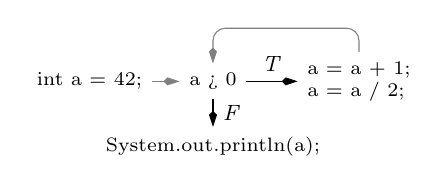
\begin{tikzpicture}[Rect/.append style={font=\scriptsize,align=left}]
\node[Rect] (a) {\bIndexR{int a = 42;}};
\node[Rect,right=3.5mm,rounded corners=9pt] (b) at (a.east) {\bIndexR{a > 0}};
\node[Rect,right=6.5mm] (c) at (b.east) {\bIndexR{a = a + 1;}\\\bIndexR{a = a / 2;}};
\node[Rect,below=3.5mm,double] (d) at (b.south) {\bIndexR{System.out.println(a);}};
\draw[-Kite,gray] (a) -- (b);
\draw[-Kite] (b) to[edge node={node[above] {\footnotesize\textit{T}}}] (c);
\draw[-Kite] (b) to[edge node={node[right] {\footnotesize\textit{F}}}] (d);
\draw[rounded corners=4.5pt,gray,-Kite] (c.north) -- ++(0,3mm) -| (b.north);
\end{tikzpicture}
\end{lrbox}
\begin{frame}[fragile]{A Best Friend for Life: Control Flow Graph (CFG)\;\supercite{cooper2022engineering}}
\begin{onlyenv}<6-|handout:1>
\begin{lrbox}{\SimpleCFG}
\figureversion{lf}\selectfont
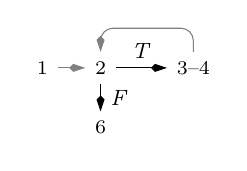
\begin{tikzpicture}[Rect/.append style={font=\scriptsize,align=left}]
\node[Rect] (a) {1};
\node[Rect,right=3.5mm,rounded corners=9pt] (b) at (a.east) {2};
\node[Rect,right=6.5mm] (c) at (b.east) {3--4};
\node[Rect,below=3.5mm,double] (d) at (b.south) {6};
\draw[-Kite,gray] (a) -- (b);
\draw[-Kite] (b) to[edge node={node[above] {\footnotesize\textit{T}}}] (c);
\draw[-Kite] (b) to[edge node={node[right] {\footnotesize\textit{F}}}] (d);
\draw[rounded corners=4.5pt,gray,-Kite] (c.north) -- ++(0,3mm) -| (b.north);
\end{tikzpicture}
\end{lrbox}
\global\setbox\SimpleCFG=\box\SimpleCFG
\end{onlyenv}
\begin{tikzpicture}
   \onslide<2->{
   \node[Rect,align=left,font=\small,text width=6.5cm] (@cfg) {%
       \textbf{Control Flow Graph (CFG)}\\[.125em]
       Directed graph representing all possible execution paths of a program.
       Usually uses \textit{basic blocks} as nodes.
   };}
   \onslide<3->{
   \node[below right=3mm,yshift=-3mm,xshift=2mm,align=left,Rect,font=\footnotesize,text width=5.5cm] (@basic-block-def) at(@cfg.south west) {%
       \textbf{Basic Block}\\[.125em]
       A sequence of instructions with a single entry point (no jumps in) and a single exit point (no jumps out except at the end).
   };
   \draw[gray,semithick,-Kite] ([xshift=5mm]@cfg.south west) to[bend right=20] ([xshift=4mm]@basic-block-def.north west);
   }
\end{tikzpicture}
\begin{tikzpicture}[overlay,remember picture]
   \begin{uncoverenv}<4->
      \node[Rect,above left=1.5mm,text width=3.8cm,xshift=-1cm,inner ysep=-1.75pt] at(current page.east) {\lstfs{8}
\xlstsetmintedstyle{plain number}
\begin{minted}{java}
int a = 42;
while(a > 0) {
   a = a + 1;
   a = a / 2;
}
System.out.println(a);
\end{minted}
      };
   \end{uncoverenv}
\onslide<5->{
   \node[below left=3.5mm,xshift=-1cm,Rect,inner sep=5.5pt]
      (@c) at(current page.east) {\usebox\SimpleCFG};
   \node[below right] at(@c.south west) {\scriptsize\textsb{CFG}};
}
\onslide<6->{
   \node[above right,yshift=4mm,font=\tiny,gray] at(current page.south west) {%
      \cite{cooper2022engineering}~\fullcite{cooper2022engineering}
   };
}
\end{tikzpicture}
\end{frame}

\begin{frame}[fragile]{Exercise: Build a CFG}
\lstfs{9}
\begin{uncoverenv}<2->
\begin{minipage}{.6\linewidth}   
\xlstsetmintedstyle{plain number}
\AnimateCode{%
   onslide={o2:{3,...,12},-,-,-,-,-,-,-,-,-,-,-,-,-,-,-},
   first slide=3,
   handout={3/1,4/2}
}
\begin{minted}{java}
static int gcdBad(int a, int b) {
   int i;
   if (a < b) 
        { i = a; }
   else { i = b; }
   for (;i > 1; 
            i--) {
      if (a % i == 0 && b % i == 0) {
         return i;
      }
   }
   return 1;
}
\end{minted}
\endAnimateCode
\end{minipage}
\end{uncoverenv}
\begin{lrbox}{\SimpleCFG}
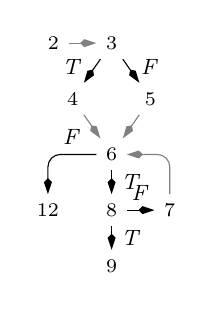
\begin{tikzpicture}[Rect/.append style={font=\scriptsize,align=left}]
\onslide<5->{
   \node[Rect] (a) {2};
}
% TODO: animate
\onslide<6->{
   \node[Rect,right=3.5mm,rounded corners=9pt] (b) at (a.east) {3};
}rounded corners=4.5pt,
\onslide<7->{
   \draw[-Kite,gray] (a) -- (b);
}
\onslide<8->{
   \node[Rect,below right=3mm] (c) at (b.south) {5};
   \node[Rect,below left=3mm] (d) at (b.south) {4};
   \draw[-Kite] (b) to[edge node={node[right,yshift=.5mm] {\footnotesize\textit{F}}}] (c);
   \draw[-Kite] (b) to[edge node={node[left,yshift=.5mm] {\footnotesize\textit{T}}}] (d);
}
\onslide<9->{
   \node[Rect,below=3mm,rounded corners=9pt] (i) at (b.south|-c.south) {6};
   \draw[-Kite,gray] (c) -- (i);
   \draw[-Kite,gray] (d) -- (i);
},gray
\onslide<10->{
   \node[Rect,below=3mm,rounded corners=9pt] (e) at (i.south) {8};
   \draw[-Kite] (i) to[edge node={node[right] {\footnotesize\textit{T}}}] (e);
}
\onslide<11->{
   \node[Rect,right=3.5mm] (h) at (e.east) {7};
   \draw[-Kite] (e) to[edge node={node[above] {\footnotesize\textit{F}}}] (h);
}
\onslide<12->{
   \draw[rounded corners=4.5pt,gray,-Kite] (h.north) |- (i.east);
}
\onslide<13->{
   \node[Rect,below=3mm,double] (g) at(e.south) {9};
   \draw[-Kite] (e) to[edge node={node[right] {\footnotesize\textit{T}}}] (g);
}
\onslide<14->{
   \node[Rect,left=3.5mm,double] (f) at (e.west) {12};
   \draw[rounded corners=4.5pt,-Kite] (i) -| (f.north) node[pos=0.25,above] {\footnotesize\textit{F}};
}
\end{tikzpicture}
\end{lrbox}
\begin{tikzpicture}[overlay,remember picture]
\onslide<4-|handout:2>{ 
   \node[left=3.5mm,xshift=-1cm,Rect,inner sep=5.5pt]
      (@c) at(current page.east) {\usebox\SimpleCFG};
   \node[below right] at(@c.south west) {\scriptsize\textsb{CFG}};
}
\onslide<15->{
   \node[above=7.5mm,text width=8cm,font=\footnotesize] at(current page.south) {%
     \begin{itemize}
         \item How to find dead code?\\
               \onslide<16-|handout:2>{E.g., nodes not reachable from the start node.}
         \item<17-> How to find infinite loops?\\
               \onslide<18-|handout:2>{E.g., nodes that cannot reach an exit node.}
     \end{itemize} 
   };
}
\end{tikzpicture}
\end{frame}

\subsection{Data and Control Flow Analyses}
\savebox\PinguBox{\tikz{\pingu[hat,eyes wink,right wing wave,lollipop left=red]; \node[above] at (pingu-wing-right-tip) {\huge\faQuestion};}}
\newsavebox\AnomaliesFM
\begin{frame}{Using the CFG: Find Dataflow Anomalies}
\begin{itemize}
   \itemsep8pt
   \item<2-> For every variable, we record the following actions: \begin{itemize}
      \item<3-> \parbox{.75\linewidth}{\parbox{1ex}{\textbf{d}} Definition (write)\hfill\textcolor{gray}{\texttt{x = 42}}}
      \item<4-> \parbox{.75\linewidth}{\parbox{1ex}{\textbf{r}} Reference (read) \hfill\textcolor{gray}{\texttt{print(x)}}}
      \item<5-> \parbox{.75\linewidth}{\parbox{1ex}{\textbf{u}} Undefined (before write, end of program,~\ldots)\hfill\textcolor{gray}{\texttt{int x}}}
   \end{itemize}
   \item<6-> Following the CFG \begin{itemize}
      \item<7-> we track the state of each variable,
      \item<8-> iterate on control-flow cycles \textcolor{gray}{until reaching a fixed point,}
      \item<9-> go statement-by-statement for basic blocks,
      \item<10-> and report anomalies.
   \end{itemize}
\end{itemize}
\only<12->{
   \vspace*{8em}
}
\begin{lrbox}{\AnomaliesFM}
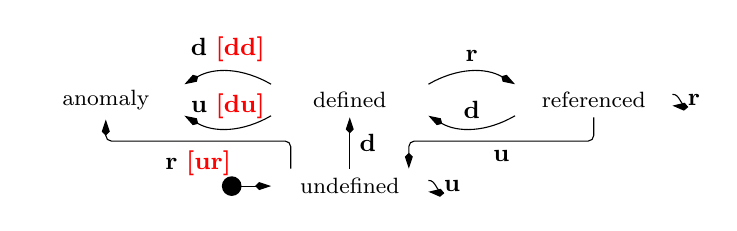
\begin{tikzpicture}[Rect/.append style={font=\footnotesize,align=center,text width=1.75cm}]
   \node[Rect] (u) at(0,0) {undefined};
   \fill ([xshift=-5mm]u.west) circle[radius=1.25mm];
   \draw[-Kite] ([xshift=-5mm]u.west) -- (u.west);
   \draw[-Kite] ([yshift=-1.5mm]u.north east) to[out=5,in=-5,looseness=1.75, edge node={node[right,pos=.5] {\small\textbf{u}}}] ([yshift=1.5mm]u.south east);
   \onslide<14->{
      \node[Rect,above=6.5mm] (d) at(u.north) {defined};
      \draw[-Kite] (u.north) -- (d.south) node[pos=.5,right] {\small\textbf{d}};
   }
   \onslide<15->{
      \node[Rect,right=11mm] (r) at(d.east) {referenced};
      \draw[-Kite,rounded corners=2pt] (r.south) -- ++(0,-3mm) coordinate (@x) -| ([xshift=7.5mm]u.north)
      node[pos=.25,below] {\small\textbf{u}};
      \draw[-Kite] ([yshift=-1.5mm]r.north east) to[out=5,in=-5,looseness=1.75, edge node={node[right,pos=.5] {\small\textbf{r}}}] ([yshift=1.5mm]r.south east);
   }
   \onslide<16->{
      \draw[-Kite] ([yshift=2mm]d.east) to[bend left,
         edge node={node[above,pos=.5] {\small\textbf{r}}}
      ] ([yshift=2mm]r.west);
      \draw[-Kite] ([yshift=-2mm]r.west) to[bend left,
         edge node={node[above,pos=.5] {\small\textbf{d}}}
      ] ([yshift=-2mm]d.east);
   }
   \onslide<17->{
      \node[Rect,double,left=11mm] (a) at(d.west) {anomaly};
      \draw[-Kite,rounded corners=2pt] ([xshift=-7.5mm]u.north) coordinate (@) -- (@x-|@) -| (a.south) node[pos=.25,below] {\small\textbf{r} \textcolor{red}{\textbf{[ur]}}};
   }
   \onslide<18->{
      \draw[-Kite] ([yshift=2mm]d.west) to[bend right,
         edge node={node[above,pos=.5] {\small\textbf{d} \textcolor{red}{\textbf{[dd]}}}}
      ] ([yshift=2mm]a.east);
   }
   \onslide<19->{
      \draw[-Kite] ([yshift=-2mm]d.west) to[bend left,
         edge node={node[above,pos=.5] {\small\textbf{u} \textcolor{red}{\textbf{[du]}}}}
      ] ([yshift=-2mm]a.east);
   }
\end{tikzpicture}
\end{lrbox}
\global\setbox\AnomaliesFM=\box\AnomaliesFM
\begin{tikzpicture}[overlay,remember picture]
   \onslide<11->{
      \node[above left=.5mm,yshift=3.5mm] (@) at(current page.south east) {\scalebox{.5}{\usebox\PinguBox}};
      \node[below left=1.5mm,xshift=2.75mm] (@) at (@.north west) {%
         Anomalies?
      };   
   }
   \onslide<13->{
      \node[above=6.25mm,xshift=-1.5cm] at(current page.south) {\scalebox{.95}{\usebox\AnomaliesFM}};
   }
\end{tikzpicture}
\end{frame}

\begin{lrbox}{\SimpleCFG}
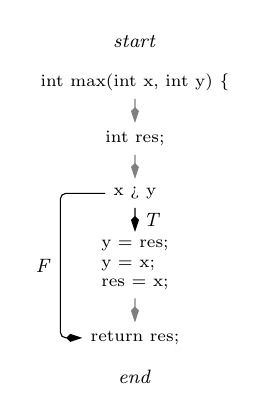
\begin{tikzpicture}[Rect/.append style={font=\scriptsize,align=left},remember picture,scale=.875,every node/.style={transform shape}]
\node[Rect] (a) {\bIndexR{int max(int x, int y) \{}};
\node[above=1.25mm] (start) at(a.north) {\footnotesize\textit{start}};
\node[Rect,below=3.5mm] (b) at (a.south) {\bIndexR{int res;}};
\node[Rect,below=3.5mm,rounded corners=7.5pt] (c) at (b.south) {\bIndexR{x > y}};
\node[Rect,below=3.5mm] (d) at (c.south) {%
   \bIndexR{y = res;}\\
   \bIndexR{y = x;}\\
   \bIndexR{res = x;}
};
% return
\node[Rect,below=3.5mm,double] (e) at (d.south) {\bIndexR{return res;}};
\node[below=1.25mm] (end) at(e.south) {\footnotesize\textit{end}};
\draw[-Kite,gray] (a) -- (b);
\draw[-Kite,gray] (b) -- (c);
\draw[-Kite] (c) to[edge node={node[right] {\footnotesize\textit{T}}}] (d);
\draw[-Kite,rounded corners=2pt] (c.west) -- ++(-6.5mm,0) |- (e.west) node[pos=0.25,left] {\footnotesize\textit{F}};
\draw[-Kite,gray] (d) -- (e);
% TODO continue
\end{tikzpicture}
\end{lrbox}
\begin{frame}{Let's Run an Example!}
\begin{tikzpicture}[overlay,remember picture]
   \node[below left=2.25mm] (@) at(current page.north east) {\scalebox{.9}{\usebox\AnomaliesFM}};
   \onslide<2->{
      \node[right=1cm,yshift=-7.5mm] (@c) at(current page.west) {\usebox\SimpleCFG};
   }
   \onslide<3->{
      \node[above right=4mm,yshift=-3.25mm] (@x) at(@c.north east) {\bfseries\texttt{x}};
      \node[right=4mm] (@y) at(@x.east) {\bfseries\texttt{y}};
      \node[right=4mm] (@res) at(@y.east) {\bfseries\texttt{res}};
   }
   \onslide<4->{
      \node at(start-|@x) {u};
      \node at(start-|@y) {u};
   }
   \onslide<5->{
      \node at(a-|@x) {d};
      \node at(a-|@y) {d};
   }
   \onslide<6->{
      \node (ur1) at(b-|@res) {u};
   }
   \onslide<7->{
      \node at(c-|@x) {r};
      \node at(c-|@y) {r};
   }
   \onslide<8->{
      \coordinate[yshift=3.5mm] (mark@ul) at(d-|@x);
      \node[yshift=3.5mm] (ur2) at(d-|@res) {r};
      \node[yshift=3.5mm] (dd1) at(d-|@y) {d};
   }
   \onslide<9->{
      \node (dd2) at(d-|@y) {d};
      \node at(d-|@x) {r};
   }
   \onslide<10->{
      \node[yshift=-3.5mm] at(d-|@res) {d};
      \node[yshift=-3.5mm] at(d-|@x) {r};
      \coordinate (mark@lr) at ([yshift=-3.5mm]d-|@res);
   }
   \onslide<11->{
      \node (bur2) at(e-|@res) {r};
   }
   \onslide<12->{
      \node at(end-|@res) {u};
      \node at(end-|@x) {u};
      \node (du2) at(end-|@y) {u};
   }
   % we also have to consider both positions
   \onslide<13->{
      \draw[gray,thick,rounded corners=4pt]
         ([xshift=-3mm,yshift=3mm]mark@ul)
            node[above right,yshift=-.5mm] {\scriptsize\textbf{True}}
            rectangle
         ([xshift=3mm,yshift=-3mm]mark@lr);
   }
   \pgfonlayer{background}
   \onslide<14->{
      \draw[thick,rounded corners=4pt,red,fill=red,fill opacity=.15]
         (dd1.north west)
            rectangle
         (dd2.south east);
   }
   \onslide<16->{
      \draw[thick,rounded corners=4pt,red,fill=red,fill opacity=.15]
         ([xshift=-1mm,yshift=-1mm]dd2.north west)
            rectangle
         ([xshift=1mm]du2.south east);
   }
   \onslide<18->{
      \draw[thick,rounded corners=4pt,red,fill=red,fill opacity=.15]
         (ur1.north west)
            rectangle
         (ur2.south east);
   }
   \onslide<20->{
      \draw[thick,rounded corners=4pt,red,fill=red,fill opacity=.15]
         ([xshift=-1mm,yshift=1mm]ur1.north west) coordinate (@)
           -| ([xshift=4mm,yshift=-1mm]bur2.south east)
           -| ([xshift=-1mm]bur2.north west)
           -| ([xshift=1.5mm]ur1.south east)
           -| ([yshift=-3mm]@) -- cycle;
   }
   \endpgfonlayer
   \node[left=6mm,text width=6.5cm,yshift=-1cm,font=\small] at(current page.east) {%
      \begin{itemize}
         \item<15-> \parbox{2.5em}{\textbf{\textcolor{red}{[dd]}}:} Unnecessary definition
         \item<17-> \parbox{2.5em}{\textbf{\textcolor{red}{[du]}}:} Definition without ref.
         \item<19-> \parbox{2.5em}{\textbf{\textcolor{red}{[ur]}}:} Ref. without prior definition
         \item<21> Consider all paths through the CFG!
      \end{itemize}
    };
   % TODO: also consider F path to the right
\end{tikzpicture}
% TODO: show cFG already, run through, then explain anomalies: dd, du, ur
\end{frame}

\subsection{Abstract Interpretation}

\begin{frame}{Reality Is \textit{\color{lightgray}more} Complex, Ain't It?}
   \begin{itemize}
      \itemsep8pt
      \item<2-> Languages possess many features \vspace*{-.85\baselineskip}
      \begin{multicols}{2}
      \begin{itemize}
         \item<3-> Concurrency\supercite{9406024}
         \item<4-> Reflection\supercite{10.1145/3426470}
         \item<5-> Dynamic loading\supercite{10.1145/3652892.3700761}
         \item<6-> Native calls\supercite{10.1145/3691620.3696193}
         \item<7-> Exceptions\supercite{JO200459}
         \item<7-> \ldots
      \end{itemize}
      \end{multicols}
      \item<8-> These features usually intertwine with each other
      \item<9-> A plethora of techniques try to address these challenges from various perspectives
      \item<10-> One prominent technique is \textit{abstract interpretation}\supercite{cousout2021principles}\\[-2.5pt]
         \textcolor{gray}{\footnotesize\itshape We'll tackle this in the second lecture!}
   \end{itemize}
\end{frame}


\section{Important Terminology}

\begin{frame}{Let's Return to the Roots}
\begin{center}
   \onslide<2->{\large Discover \textit{syntactic/semantic properties} of programs\\\textsb{without} running them.}
\end{center}
\vspace*{3em}

\begin{itemize}
   \item<3-> Depending on our focus, we are interested in: \begin{itemize}
      \itemsep5.5pt
      \item<4-> Satisfying these properties (\textsb{verification})\\[-2.5pt]
         \onslide<5->{\textcolor{gray}{\footnotesize\itshape E.g., \textit{x is always non-negative}}}
      \item<6-> Violating these properties (\textsb{bug finding})\\[-2.5pt]
         \onslide<7->{\textcolor{gray}{\footnotesize\itshape E.g., \textit{possible division by zero}}}
   \end{itemize}
\end{itemize}
\end{frame}

\newsavebox\LeslieLamport
\savebox\LeslieLamport{%
\ImageWithRoundedCorners{22.5mm}{leslie-lamport.jpg}%
}
\newsavebox\FloLeslie
\savebox\FloLeslie{%
\ImageWithRoundedCorners{72.5mm}{flo-leslie.jpg}%
}
\begin{frame}{Liveness and Safety Properties\;\supercite{rival2020introduction,lamport1977proving}}
   \begin{itemize}
      \itemsep16pt
      \item<2-> \textbf{Liveness properties:} (\enquote{good things}, infinite time)\\
               Things that \textit{must} happen during execution. \textcolor{lightgray}{\textit{For example,}}
               \begin{itemize}
                  \item<3-> Every request eventually receives a response.
                  \item<4-> Every thread that is started eventually terminates.
                  \item<5-> \ldots
               \end{itemize}
            
      \item<6-> \textbf{Safety properties:} (\enquote{bad things}, finite time)\\
               Things that \textit{must not} happen during execution. \textcolor{lightgray}{\textit{For example,}} 
               \begin{itemize}
                  \item<7-> Integer variables never overflow.
                  \item<8-> Array accesses are always within bounds.
                  \item<9-> \ldots
               \end{itemize}
   \end{itemize}
   \begin{tikzpicture}[overlay,remember picture]
      \onslide<11->{
         \node[below left=2.65mm,align=right,font=\tiny,
         ] at(current page.north east) {%
            \usebox\LeslieLamport\\[1.65pt]
            \textsb{Leslie B. Lamport (1941)}\kern2pt\\%
            \color{gray}Heidelberg Laureate Forum\kern2pt
         }; 
         \node[above left=1.25mm,yshift=3.5mm] at(current page.south east) {\scalebox{.5}{\usebox\FloLeslie}};
      }  
   \end{tikzpicture}
\end{frame}
\newsavebox\pinguA
\savebox\pinguA{\tikz{\pingu[wings grab,eyes sad,cup=red,wool hat]}}
\subsection{Soundness and Completeness}
\newsavebox\HenryRice
\savebox\HenryRice{%
\ImageWithRoundedCorners{18.25mm}{henry-rice.jpg}%
}
\begin{frame}{Rice's Theorem}
   \begin{itemize}
      \itemsep12pt
      \item<2-> We want to prove properties of programs\\
           (e.g., no overflow, shapes,~\ldots)
      \item<3-> However, thanks to \citeauthor{rice1953classes}~\cite{rice1953classes} we know:\smallskip\\
      \begin{quote}<4->
         Rice's theorem states that all nontrivial semantic properties of programs are undecidable.~\cite[100]{cousout2021principles}
      \end{quote}
      \item<5-> We can not solve the halting problem
      \item<6-> We have to approximate the reality
   \end{itemize}
\begin{tikzpicture}[overlay,remember picture]
   \onslide<5->{\node[above left=.5mm,yshift=3.5mm] at(current page.south east) {\scalebox{.5}{\usebox\pinguA}};}
   \onslide<4->{
      \node[below left=4.65mm,align=right,font=\tiny,
         href node={https://medium.com/@shreeshail.chitpur21/rices-theorem-c77540af3693}
      ] at(current page.north east) {%
         \usebox\HenryRice\\[1.65pt]
         \textsb{Henry Gordon Rice (1920--2003)}\kern2pt\\%
         \color{gray}Medium\kern2pt
      }; 
   }
\end{tikzpicture}
\end{frame}

\def\Box#1{\parbox{2cm}{\centering#1}}
\def\mark{\color{green}\bfseries}
\begin{frame}{The Confusion Matrix (Reminder)}
   \centering
   \begin{tabular}{c@{\hskip9pt}lcc}
      & & \multicolumn{2}{c}{\onslide<2->{\tikzmarknode{prediction}{\textsb{Prediction}}}} \\
      & & \onslide<3->{\textsb{Pos.}} & \onslide<4->{\textsb{Neg.}} \\[2mm]
      \multirow{2}{*}{\onslide<5->{\tikzmarknode{actual}{\rotatebox[origin=c]{90}{\textsb{Actual}\kern9pt}}}} 
      & \onslide<6->{\textsb{Pos.}} & \onslide<8->{\mark \Box{(TP) True Positive}} & \onslide<9->{\Box{(FN) False Negative}} \\[6mm]
      & \onslide<7->{\textsb{Neg.}} & \onslide<10->{\Box{(FP) False Positive}} & \onslide<11->{\mark\Box{(TN) True Negative}}
   \end{tabular}
   \begin{tikzpicture}[overlay,remember picture,gray,line cap=round]
      \onslide<2->{\draw[Kite-] ([yshift=2pt]prediction.north) to[out=80,in=190] ++(1,.5) node[right,font=\scriptsize] {E.g., do we claim there is an error?};}
      \onslide<5->{
         \draw[Kite-] ([xshift=-1.5pt]actual.west) to[out=180,in=80] ++(-.4,-1.2) node[below,font=\scriptsize] {E.g., is there really an error?};
      }
   \end{tikzpicture}
   \vspace*{2.45em}
   \begin{itemize}
      \item<12-> \parbox{1.8cm}{\strut\textsb{Precision:}} \(\text{\mark TP} / (\text{\mark TP} + \text{FP})\) \quad \textcolor{gray}{(\enquote{how many false alarms})}
      \item<13-> \parbox{1.8cm}{\strut\textsb{Recall:}} \(\text{\mark TP} / (\text{\mark TP} + \text{FN})\) \quad \textcolor{gray}{(\enquote{how many errors did we find})}
   \end{itemize}
   \note[itemize]{
      \item False positive ist Type I
      \item False negative ist Type II
   }
\end{frame}

\begin{frame}{Soundness and Completeness}
   \onslide<2->{\textbf{Soundness} \textcolor{gray}{\footnotesize(\enquote{Correct Over-Approximation})}}\vspace*{-2mm}
   \begin{itemize}
      \item<3-> All properties we derive are true (but we may miss some)
      \item<4-> If we report bugs for violated properties, we produce no false negative
   \end{itemize}
   \bigskip

   \onslide<5->{\textbf{Completeness} \textcolor{gray}{\footnotesize(\enquote{Correct Under-Approximation})}}\vspace*{-2mm}
   \begin{itemize}
      \item<6-> We are able to infer all interesting properties in the program
      \item<7-> If we report bugs for violated properties, we produce no false positive
   \end{itemize}

   \note[itemize]{
      \item Sound: Vlt. sagen wir es gibt wo ein problem, wo es keins gibt, soundiness: restrict to some features
      \item Complete: Vlt. sagen wir es gibt kein problem, wo es eins gibt
   }
\end{frame}

\begin{frame}[c]{What is Sound, What is Complete?}
\centering
\begin{tikzpicture}
   \onslide<2->{\node[Rect,align=left,font=\small,text width=5cm] (@t) {%
      \strut\textbf{Testing}\\[.125em]
      {\onslide<3-|handout:2>{Complete, but unsound.}}\\
      {\onslide<4-|handout:2>{\parbox{4.9cm}{\scriptsize\itshape We find definitely reachable states, but (generally) not all!\strut\endgraf}}}
   };}
   \onslide<5->{\node[Rect,align=left,font=\small,text width=5cm,right=5mm] (@fmc) at (@t.east) {%
      \strut\textbf{Finite Model Checking}\\[.125em]
      {\onslide<6-|handout:2>{Complete and sound.}}\\
      {\onslide<7-|handout:2>{\parbox{4.9cm}{\scriptsize\itshape
       Explore \textit{all} states in a \textit{finite} model, but the model may wrongly represent reality.\strut
      \endgraf}}}
   };}
   \onslide<8->{
   \node[Rect,align=left,font=\small,text width=5cm,below=5mm] (@si) at (current bounding box.south) {%
      \strut\textbf{Static Analysis}\\[.125em]
      {\onslide<9-|handout:2>{Sound, but incomplete.}}\\
      {\onslide<10-|handout:2>{\parbox{4.9cm}{\scriptsize\itshape We find \textit{all} runtime states in an \textit{abstract} model, but may over-approximate.\strut\endgraf}}}
   };}
\end{tikzpicture}
\vspace*{1em}\footnotesize
\begin{itemize}
   \item<11-|handout:1-> What is more important? \onslide<12->{Depends on what you want!} \begin{itemize}
     \itemsep4pt
      \item<13-|handout:1-> \footnotesize Make sure the auto-pilot cannot steer directly down? \\[-1.5pt]
      \onslide<14-|handout:2>{Soundness is key.}
      \item<14-|handout:1-> \footnotesize Need to show your website can be viewed?\\[-3pt]
      \onslide<15-|handout:2>{You better want completeness.}
   \end{itemize}
\end{itemize}
\end{frame}

\section{Outlook}

\begin{frame}{A Couple of Questions to Round It Of}
\begin{enumerate}
   \itemsep=12pt
   \item<2-> How would you capture what a \textit{property} is?
   \item<3-> How would you phrase that one property is \enquote{better} than another?
   \item<4-> For what operations would you \textit{not} use a control-flow graph?
   \item<5-> Why can't there be a fully automatic, sound, and complete static analyzer for general programs?
   \item<6-> What (big) additional challenges do you see in the real-world?
\end{enumerate}
\vspace*{1.25em}
\begin{center}
   \onslide<7->{We will address these questions in the next lecture(s)!}
\end{center}
\end{frame}

% \begin{frame}
%    TODO: open hiwi opsition
% \end{frame}

\renewcommand*{\bibfont}{\tiny}

\AtBeginSection{}
\begin{frame}[allowframebreaks]{References}
   \printbibliography[title={}] % TODO
\end{frame}

\end{document}